\documentclass[12pt, a4paper,oneside]{book}
% Подключение библиотеки
\usepackage{/Users/vladbelousov/Desktop/Semestr_4-FP-NSU/Настройка/library}

\begin{document}

\begin{titlepage}
    \thispagestyle{empty}  % Отключаем нумерацию страницы на титульном листе
    \centering
    \vspace*{1cm}  % Отступ сверху

    \textbf{\huge Конспект лекций по дисциплине}  \\[1.5cm]  % Название
    \textbf{\huge Электродинамика и оптика }  \\[2cm]   % Название дисциплины (оставьте пустым для добавления вручную)
    \textbf{\Large Новосибирский государственный университет} \\[0.5cm]
    \textbf{\large Физический факультет} \\[0.5cm]
    \textbf{\large 4-й семестр} \\[0.5cm]
    \textbf{\large 2025 год} \\[10cm]

    \begin{flushright}
        \large Студент: Б.В.О \\[0.5cm]  % Ваше имя
        Преподаватель: Синицкий Станислав Леонидович  % Ф.И.О. преподавателя
    \end{flushright}
\end{titlepage}

\tableofcontents  % Создание оглавления

\def\mainfile{}  % Определяем макрос для основного файла
% Условная компиляция для самостоятельной работы
\ifdefined\mainfile
    % Если это часть основного файла, не добавляем начало и конец документа
\else
    \documentclass[12pt, a4paper]{report}
    \usepackage{/Users/vladbelousov/Desktop/Semestr_4-FP-NSU/Настройка/library}
    \usepackage[utf8]{inputenc} % Подключение поддержки UTF-8
    \begin{document}
\fi

%%-------------------------------%%

\chapter{Электромагнитные волны.}

\section{Свободное электромагнитное поле. Волновое уравнение.  }

\begin{definition}[Свободное]   
означает без токов и зарядов \( \Rightarrow \rho =0 , \vec{j}= 0   \) 
\end{definition}

\[ 
\begin{aligned}
    \begin{cases}
         \displaystyle \mathrm{rot} \vec{ E} =-\frac{1}{c}\frac{\partial\vec{B}}{\partial t}, \quad \mathrm{div} \vec{B}=0 \\
        \displaystyle \mathrm{rot} \vec{H} =\frac{1}{c}\frac{\partial\vec{D}}{\partial t}, \quad \mathrm{div} \vec{D}=0     
    \end{cases} 
    + \text{Грани. условия} 
    \text{ } 
    \begin{cases}
        (B_n)| = 0 \quad (E_{\tau} )= 0 \\ 
        (D_n)| = 0 \quad (H_{\tau} )= 0 
    \end{cases}
\end{aligned}
 \] 

 \textit{Два типа векторных полей:} 

 1. Вихревые: \( \mathrm{div}\vec{F}= 0    \)  (нет источников истоков этого поля \( \Rightarrow  \) силовые линии либо замкнуты, либо уходят на бесконечность)

\begin{center}
    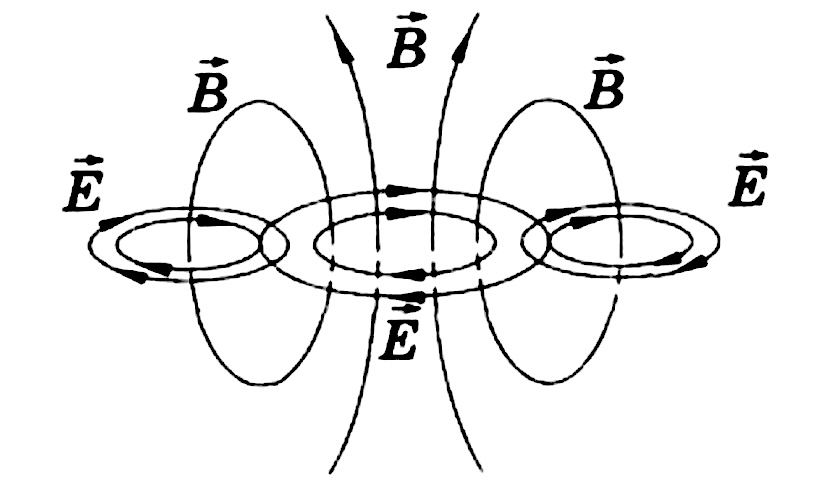
\includegraphics[width=0.3\textwidth]{/Users/vladbelousov/Desktop/Semestr_4-FP-NSU/ЭиО/Лекции_по_дням/image/1.jpeg}
\end{center}

 2. Потенциальные: \( \mathrm{rot} \vec{F} =0 \). Силовые линии выходят или входят в области стоков и истоков (где \( \mathrm{div} \vec{F} \neq 0     \)) или на бесконечности. 

\begin{center}
    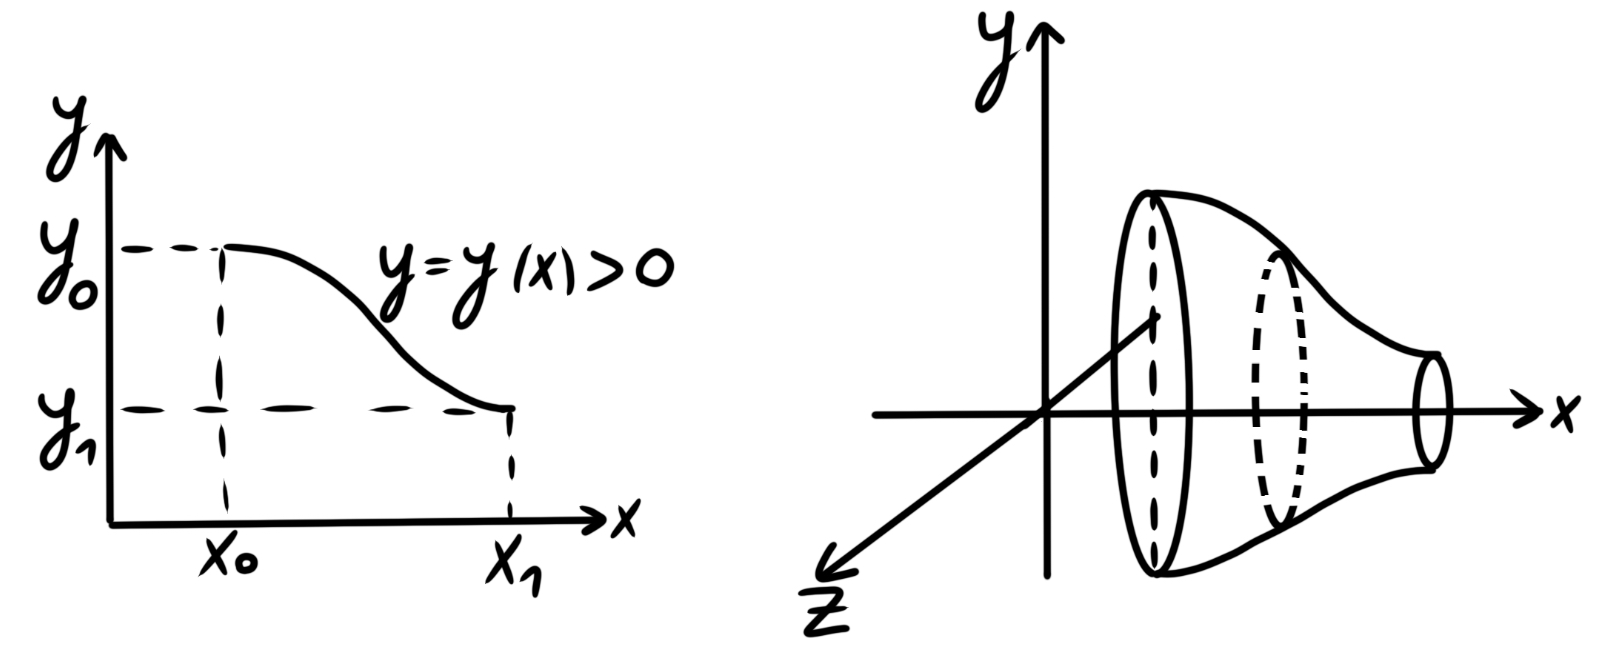
\includegraphics[width=0.5\textwidth]{/Users/vladbelousov/Desktop/Semestr_4-FP-NSU/ЭиО/Лекции_по_дням/image/2.png}
\end{center}

Далее мы будем рассматривать только вихревые поля (т.е. \( \mathrm{div} \vec{B} = 0 ,\mathrm{div} \vec{D} = 0  \))

Неизвестные 3 компоненты каждого поля: \( \vec{E},\vec{D},\vec{B},\vec{H}\) - 12 неизвестные функций. Мы можем решить эту систему при помощи уравнений Максвелла \( + \)  материальные уравнения: \( \vec{B}=\vec{B}(H), \vec{E}=\vec{E}(D) \).

Простая модель среды: \( \vec{B}=\mu\vec{H}, \vec{D}=\varepsilon \vec{E} \), где \( \mu = \mathrm{const}  , \varepsilon =\mathrm{const}   \), годится для вакуума (\(\mu=1, \varepsilon=1  \)) и для многих других сред/материалов при низких значения полей \( \vec{E}, \vec{B} \)  и при невысоких частотах \( f < 10^8 \) Гц. 
 
\newpage

\textit{Волновое уравнение:} 

Рассмотрим \(  \displaystyle  \mathrm{rot} (\mathrm{rot} \vec{E}  )= -\frac{\mu}{c}  \frac{\partial}{\partial t} \mathrm{rot } \vec{H}= - \frac{\mu \varepsilon}{ c ^2} \frac{\partial ^2}{\partial t ^2}     \vec{E} \\ \) 

Распишем чему равен \( \mathrm{rot}(\mathrm{rot}\vec{E}  )   \) :

\[         \displaystyle \mathrm{rot} (\mathrm{rot} \vec{E}  )= \nabla \underbrace{\mathrm{div} \vec{E}}_{\frac{1}{\varepsilon} \mathrm{div}\vec{D}=0   }    - \Delta \vec{E}   \] 

Получаем нашу систему:

\[
\begin{aligned}
    \begin{cases}
        \displaystyle \Delta \vec{E}- \frac{\mu \varepsilon}{c ^2} \frac{\partial ^2 \vec{E}}{\partial t ^2} =0 \\
        \displaystyle \mathrm{div}   \vec{E}=0 
    \end{cases} 
    \quad \quad  (1)
\end{aligned} 
\] 

Так же делаем с \( \mathrm{rot }(\mathrm{rot}\vec{B})\) и получаем: 

\[
\begin{aligned}
    \begin{cases}
        \displaystyle  \Delta \vec{B} - \frac{\mu \varepsilon}{c ^2} \frac{\partial ^2 \vec{B}}{\partial t ^2} =0 \\
        \displaystyle \mathrm{div}   \vec{B}=0
    \end{cases}
    \quad \quad  (2)
\end{aligned} 
\]

Согласование решений (1) и (2): 

1) Решаем (1) и \( \vec{E} \)  подстваляем в уравнение Максвелла \( \to  \vec{B} \);

2) Решаем (2) и \( \vec{B} \)  подстваляем в уравнение Максвелла \( \to  \vec{E} \);

Различные простейшие решения волнового уравнения: 

1) Плоские волны: все ненулевые компоненты полей \( \vec{ E} ,\vec{ B} \) завися от одной координаты (например от z)  и времени t; 

\begin{center}
    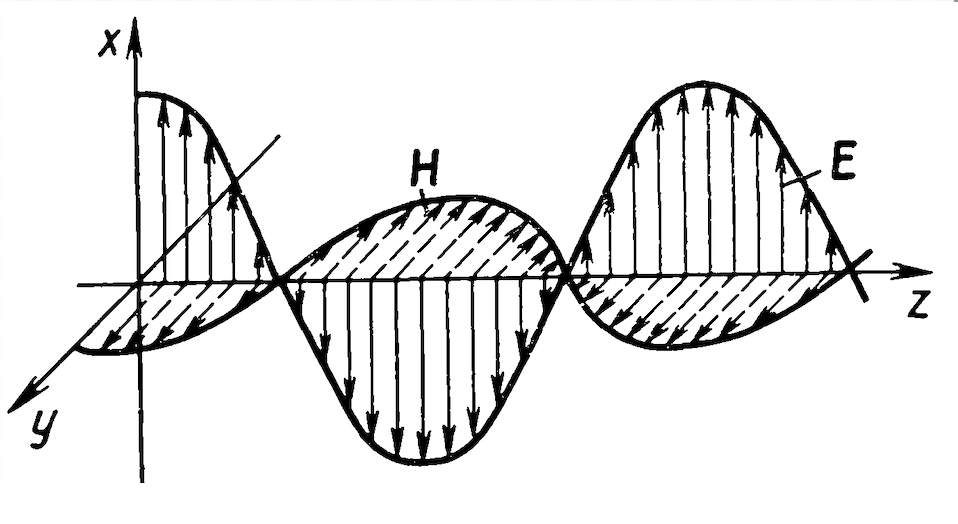
\includegraphics[width=0.3\textwidth]{/Users/vladbelousov/Desktop/Semestr_4-FP-NSU/ЭиО/Лекции_по_дням/image/3.png}
\end{center}


2) Цилиндрические волны: все ненулевые компоненты полей \( \vec{ E} ,\vec{ B} \) зависят от \( \vec{ r}  \)  - расстояния от точки наблюдения до некоторой оси (центра волны) и от времени t; 

3) Сферическая волна: все ненулевые компоненты полей \( \vec{ E} ,\vec{ B} \) зависят от \( \vec{r}  \)  - расстояния от точки наблюдения до центра волны.

\begin{center}
    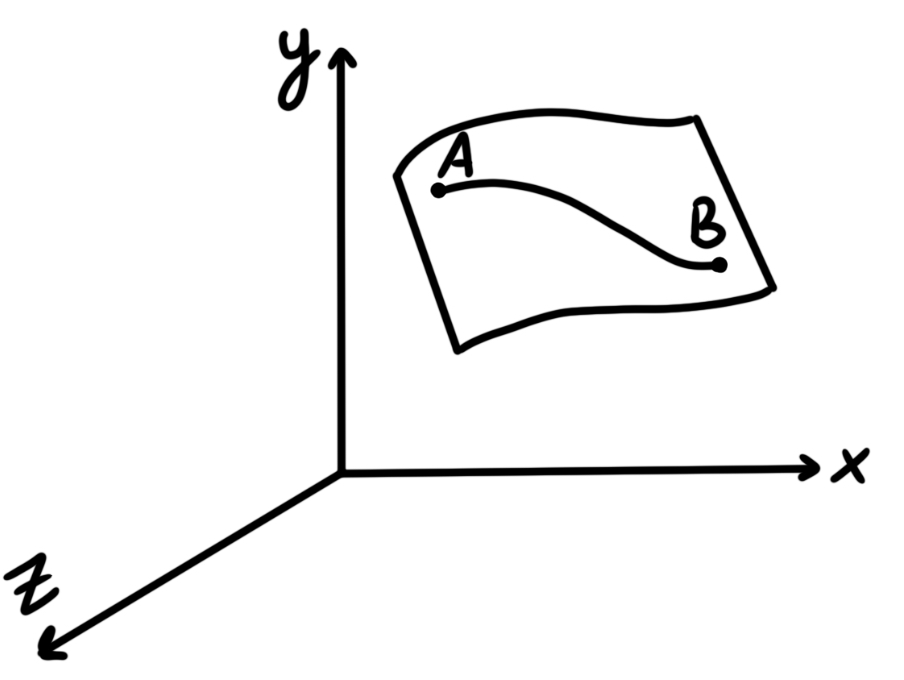
\includegraphics[width=0.3\textwidth]{/Users/vladbelousov/Desktop/Semestr_4-FP-NSU/ЭиО/Лекции_по_дням/image/4.png}
\end{center}

\newpage

\section{Плоские волны. }

\[ \frac{\partial ^2 }{\partial t^2 } \vec{E} - \frac{\mu \varepsilon}{c ^2} \frac{\partial ^2 \vec{ E}}{\partial t ^2 } =0 \text{ , для примера }  E_x : \left( \frac{\partial}{\partial z} - \frac{\sqrt{\mu \varepsilon} }{c} \frac{\partial}{\partial t }   \right) \left( \frac{\partial}{\partial z} + \frac{\sqrt{\mu \varepsilon} }{c} \frac{\partial}{\partial t } \right) E_x = 0  \quad  (*)  \] 

Под f подразумевается \( E_x  \) или \( E_y \)  

\begin{gather*}
    \xi = z - \frac{c t}{ \sqrt{\mu \varepsilon} }, \quad \eta = z + \frac{c t}{ \sqrt{\mu \varepsilon} } \quad ( \text{замена переменных} )  \\
    \frac{\partial}{\partial z } f ( \xi ( z,t), \eta(z,t) ) = \frac{\partial f}{\partial \xi }  \underbrace{\frac{\partial \xi }{\partial z }}_{=1} + \frac{\partial f }{\partial \eta  }   \underbrace{\frac{\partial \eta }{\partial z }}_{=1}= \frac{\partial f}{\partial \xi } + \frac{\partial f}{ \partial \eta } \\
    \frac{\sqrt{\mu \varepsilon}}{c}  \frac{\partial f }{\partial t}      = \frac{\sqrt{\mu \varepsilon}}{c} \left( \frac{\partial f }{\partial \xi } \left( - \frac{c}{\sqrt{\mu \varepsilon}}\right) + \frac{\partial f}{\partial \eta } \left( \frac{c}{\sqrt{\mu \varepsilon}}  \right)  \right)=- \frac{\partial f}{\partial \xi } + \frac{\partial f}{ \partial \eta }  \\ 
    \frac{\partial}{\partial z } \to  \frac{\partial}{\partial \xi } + \frac{\partial}{\partial \eta }, \quad \frac{\sqrt{\mu \varepsilon}}{c}\frac{\partial}{\partial t} \to \frac{\partial}{\partial \eta }- \frac{\partial }{\partial \xi } \\
\end{gather*} 
Подставляем в (*):

\[     \left( \frac{\partial }{\partial \xi  }+ \cancel{\frac{\partial}{\partial \eta }}  - \cancel{\frac{\partial}{\partial \eta }}  + \frac{\partial}{\partial \xi  }     \right) \left( \cancel{\frac{\partial}{\partial \xi }}  +\frac{\partial}{\partial \eta } +\frac{\partial}{\partial \eta } - \cancel{\frac{\partial}{\partial \xi }}  \right) E_x ( \varepsilon,\mu)= 0 \Rightarrow  4 \cdot \frac{\partial}{ \partial\mu \partial\varepsilon}E_x ( \varepsilon,\mu)= 0  \] 

Так как смешанные производные коммутируют ( \(\displaystyle  \frac{\partial}{\partial \mu \partial \varepsilon}= \frac{\partial}{\partial \varepsilon \partial \mu}   \)) и уравнение равно нулю, то \( \vec{E_x} \) можно представить в виде суммы двух функций.

\[     E_x (z,t) = f \left(z- \frac{c}{\sqrt{ \mu \varepsilon }}   \right)+ g \left(  z+ \frac{c}{\sqrt{ \mu \varepsilon }} \right) \\ 
\] 

Так же решения являются произвольные функции от своих аргументов: \( f(\xi) , f(\eta) \). В этом убеждают значения соответствующих вторых производных:

\[ \frac{\partial ^2 f(\xi \backslash \eta )}{ \partial z ^2} = \frac{ d ^2 f(\xi \backslash \eta )}{d (\xi \backslash \eta ) ^2}, \text{ } \frac{\partial ^2 f(\xi \backslash \eta ) }{ \partial t ^2} = \left( \pm \frac{c}{\sqrt{\mu \varepsilon}}  \right) ^2\frac{ d ^2 f(\xi \backslash \eta)}{d (\xi \backslash \eta)  ^2}   \] 

Физически это отражает принцип суперпозиции волн: любое решение может быть представлено в виде комбинации волн, движущихся в противоположных направлениях.

По аналогии можем записать \( \vec{E_y} \) :

\[ \displaystyle     E_y (z,t) = p \left(z- \frac{c}{\sqrt{ \mu \varepsilon }}   \right)+ h \left(  z+ \frac{c}{\sqrt{ \mu \varepsilon }} \right) \\ 
, \text{ где } \forall p,h  \] 


Свойства плоских волн: 

1) Из определения, что плоские волны поперечные, то-есть перпендикулярны к направлению своего движения: \( E_z = 0 , B_z =0  \).

\begin{proof}
    \[ \displaystyle  \mathrm{div}\vec{D}=\varepsilon \mathrm{div}\vec{E} =0 = \varepsilon \left( \underbrace{\frac{\partial E_x }{\partial x }}_{=0} + \underbrace{\frac{\partial E_y }{\partial y }}_{=0}+\frac{\partial E_z }{\partial z }  \right) \Rightarrow \frac{\partial \vec{E_z} }{\partial z }=0        \]

\begin{gather*}
    \mathrm{rot } \vec{H}= \frac{\varepsilon}{c} \frac{\partial \vec{E}}{\partial t} \Rightarrow \underbrace{\frac{\partial \vec{H_x}}{\partial x }}_{=0}  - \underbrace{\frac{\partial \vec{H_y}}{\partial y }}_{=0}   = \frac{\varepsilon}{c} \frac{\partial \vec{E_z} }{\partial t} \Rightarrow  \frac{\partial \vec{E_z} }{\partial t}=0
\end{gather*}

То есть все сводится к тому, что наше поле \( \vec{E_z} =E_0= \mathrm{const}\), но такое неизменное во времени однородное поле к волне отношения не имеет. Следовательно можно положить \( \vec{E_z}=0\), аналогично для \( \vec{B_z}=0 \).
\end{proof}



Пример: 

\begin{center}
    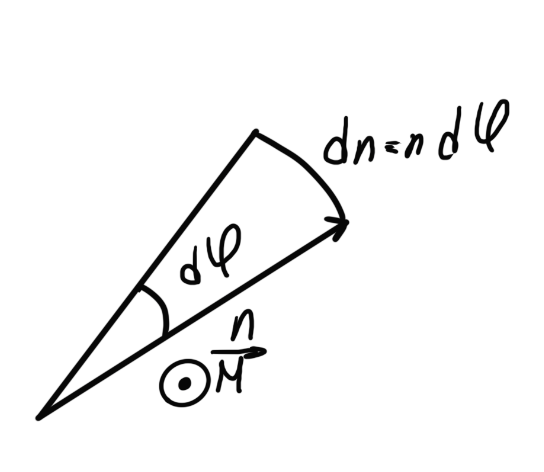
\includegraphics[width=0.7\textwidth]{/Users/vladbelousov/Desktop/Semestr_4-FP-NSU/ЭиО/Лекции_по_дням/image/5.png}
\end{center}

В максимуме \( \displaystyle z - \frac{c t}{ \sqrt{ \mu \varepsilon}} = 0   \) 

\[ \displaystyle \frac{\partial}{\partial t} \text{аргумент}=   \underbrace{\frac{dz}{dt} }_{V_{\Phi }  }- \frac{c}{\sqrt{ \mu \varepsilon}}=0   \] 

2) Связь поперечных полей в плоской волне: 

Рассмотрим бегущую волну в направлении оси z. В такой волне все величины являются функциями только от \(\displaystyle  \xi= z- \frac{c}{\sqrt{\mu \varepsilon } }t = z- ut   \) 

\[ \vec{E}= \vec{E}(\xi ) , \quad \vec{H}=\vec{H}(\xi ) \] 

Пусть \( \vec{E}= \vec{E}(\xi ) \)  произвольная функция, тогда  \(  H=H(\xi ) \) определяется из уравнения \( \displaystyle \mathrm{rot}\vec{E}= - \frac{\mu}{c} \frac{\partial \vec{H}}{\partial t}    \). Распишем левую и правую части уравнения:

\[ \mathrm{rot} \vec{E}(\xi )= \left[ \mathrm{grad} \xi \times  \frac{d \vec{E}}{d \xi }     \right]= [\vec{e_z}\times \frac{d \vec{E}}{d \xi }] = \frac{d}{d \xi  } [\vec{e_z}\times  \vec{E}(\xi )]   \] 

\[ \frac{\partial \vec{H}(\xi )}{\partial\xi }= \frac{d \vec{H}}{d\xi } \frac{\partial \xi }{\partial t}   = - u \frac{d \vec{H}}{d \xi } \] 

Подставляем это в уравнение:

\[ 
\frac{d}{d \xi} [\vec{e_z} \times \vec{E}(\xi)] = \frac{\mu}{c} u \frac{d \vec{H}}{d \xi} 
\]

Проинтегрировав по \( \xi \) получаем и подставив \( \displaystyle u=\frac{c}{\sqrt{\mu \varepsilon }} \) 


\[ \displaystyle  \sqrt{\varepsilon} \vec{E} = \sqrt{ \mu} [\vec{H}\times \vec{n}], \quad \sqrt{\mu} \vec{H} = \sqrt{ \varepsilon} [\vec{n}\times \vec{E}] \]

где \( \vec{n } \) - единичный вектор направления движения волны (\(  \vec{E} \perp \vec{B} \perp \vec{n} \)). 

3) \( \displaystyle \varepsilon E ^2 = \mu [ \displaystyle \vec{H}\times  \vec{n }] ^2 = \mu H ^2 n ^2 = \mu H ^2 | : 8 \pi \Rightarrow W_E = \frac{\varepsilon E ^2 }{8 \pi} =\frac{\mu B ^2 }{8 \pi} = W_B  \) 

4) \( \displaystyle \vec{S}= \frac{c}{4 \pi}   [ \vec{E}\times \vec{H }] \) - плотность потока энергии (вектор Умова-Пойтинга). 

\begin{gather*}
    \displaystyle \vec{S} = \frac{c}{4 \pi} [\vec{E } \times  \sqrt{\frac{\varepsilon}{\mu} }[\vec{n }\times  \vec{E}]]= \frac{c \varepsilon}{4 \pi \sqrt{ \mu \varepsilon}} \left( \vec{n}( \vec{E}\vec{E}) - \underbrace{\vec{E}( \vec{n }\vec{E})}_{=0}   \right)= \frac{c}{\sqrt{ \mu \varepsilon}} \vec{n} \left( \underbrace{\frac{\varepsilon E ^2 }{8 \pi}}_{W_E}  +\underbrace{\frac{\mu B ^2 }{8 \pi}  }_{W_B}  \right)   
\end{gather*}

\section{Плоские монохроматические волные (ПМВ).}

\( E_x, E_y, B_x, B_y \sim e^{-i \omega t}   \) 

\text{ }

\begin{minipage}{0.5\textwidth}
    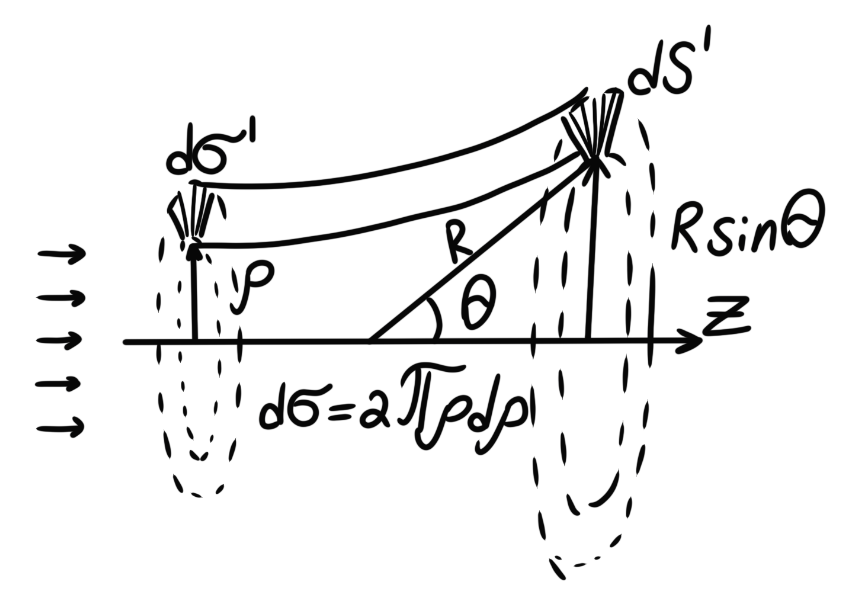
\includegraphics[width=0.5\textwidth]{/Users/vladbelousov/Desktop/Semestr_4-FP-NSU/ЭиО/Лекции_по_дням/image/6.png}
\end{minipage}
\begin{minipage}{0.5\textwidth}
    \text{В плоскости } \( z = z_0 , \vec{E}( z_0,t )= \vec{E_0}e^{-i \omega t} \Rightarrow  \) 
\end{minipage}

\begin{gather*}
    \displaystyle  \Rightarrow  \vec{E}( z,t)= \vec{E_0} e^{\frac{i \omega \sqrt{ \mu \varepsilon}}{c} \left( z- \frac{c}{\sqrt{\mu \varepsilon}} t -z_0  \right) }= \underbrace{\vec{E_0}e^{-\frac{i \omega \sqrt{ \mu \varepsilon}}{c}z_0} }_{\vec{E_{00}}} \cdot \underbrace{e^{\frac{i \omega \sqrt{ \mu \varepsilon}}{c} \left( z - \frac{c}{\sqrt{ \mu \varepsilon}}t  \right)} } _{f (z - \frac{c}{\sqrt{ \mu \varepsilon}}t)}   
\end{gather*}

\( \vec{E_0 } \perp \vec{n} = \vec{e_z} \Rightarrow \vec{E_0}=c_1 \vec{e_x}+ c_2 \vec{e_y}, c_1 \text{ и } c_2   \) - произвольные комплексные числа. 

\begin{definition}
    Волновое число \( k = \frac{\omega \sqrt{ \mu \varepsilon}}{c} = \frac{\omega}{V_{\text{волн.} } }   \) 
\end{definition}

\[ \displaystyle \vec{E}= \vec{E_{00}}e^{ikz- i \omega t } - \text{ для волны с } \vec{n} = \vec{e_z}, \qquad \vec{E}= \vec{E_{000}}e^{-ikz- i \omega t } - \text{ для волны с } \vec{n} = \vec{-e_z}  \] 

Универсальная запись полей ПМВ: 

\begin{center}
    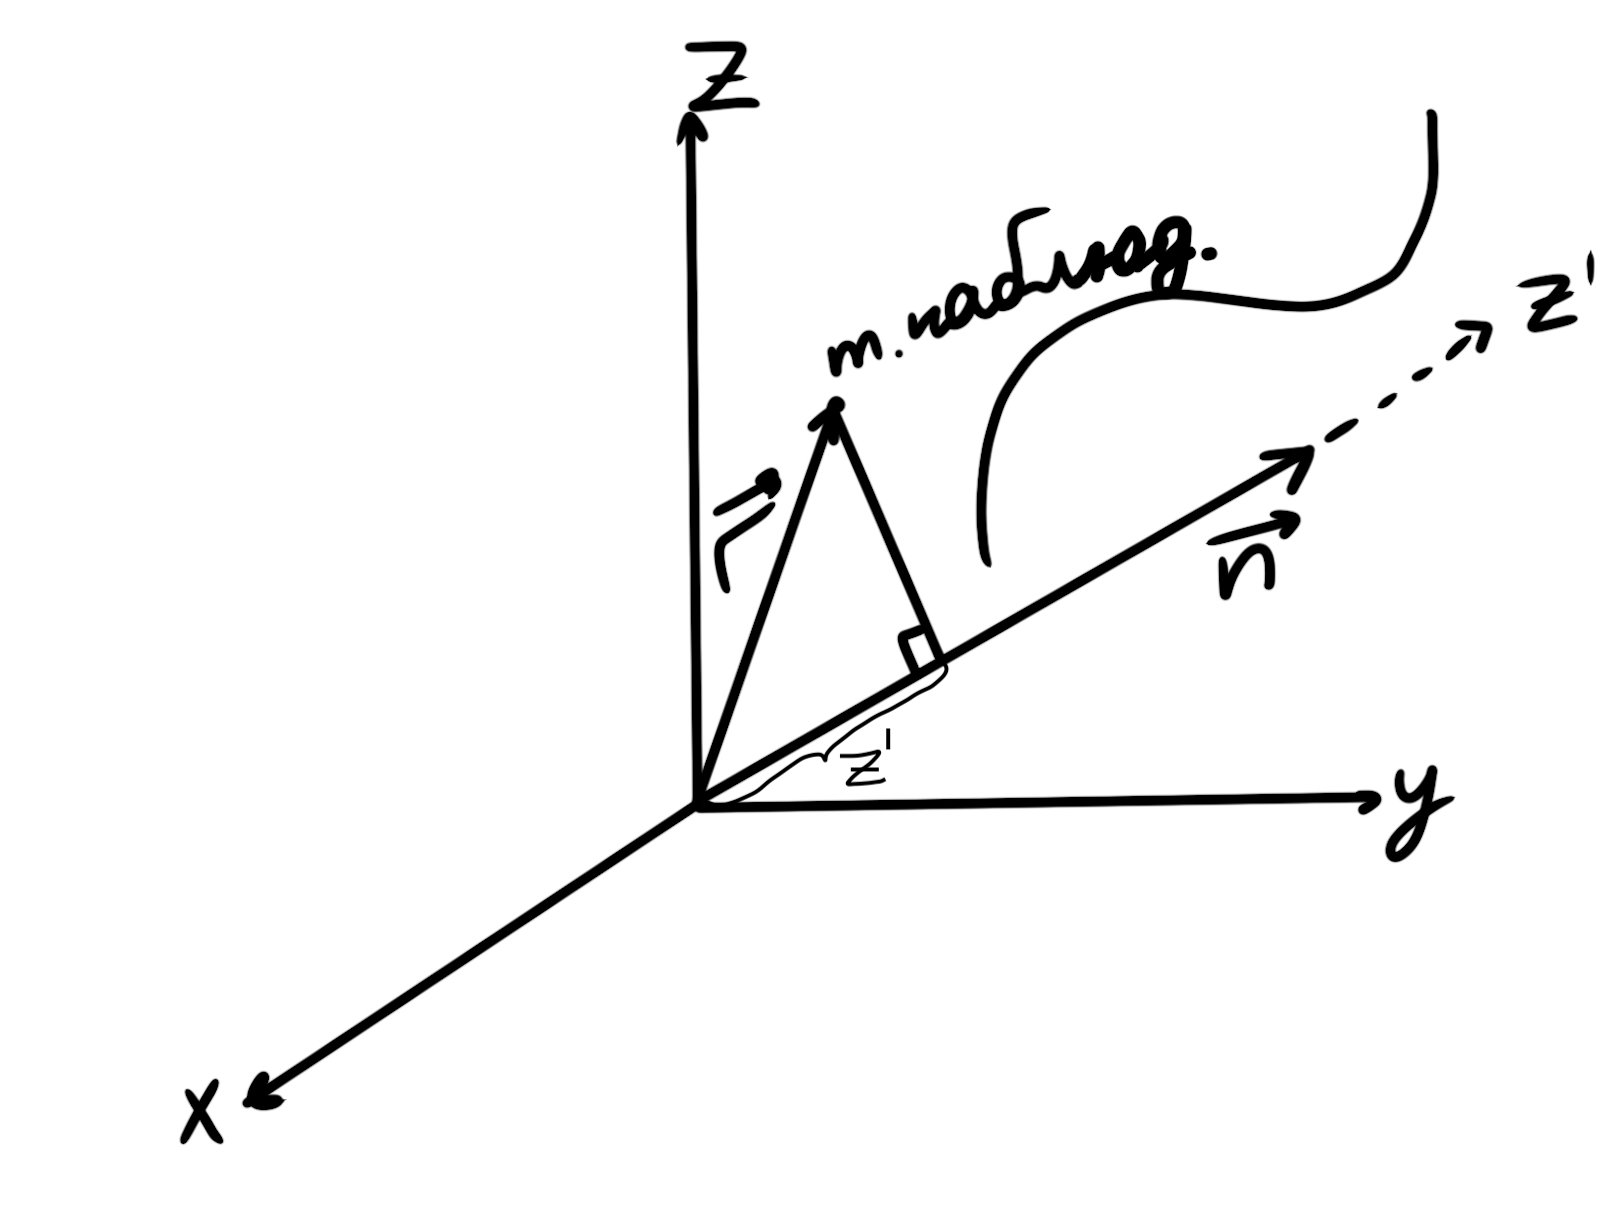
\includegraphics[width=0.3\textwidth]{/Users/vladbelousov/Desktop/Semestr_4-FP-NSU/ЭиО/Лекции_по_дням/image/7.png}
\end{center}

\[ \begin{aligned}
    \begin{cases}
        \displaystyle \vec{E}( z', t)= \vec{E_0 }e^{ikz' - i \omega t } \\  
        z'= (\vec{n}, \vec{r})
    \end{cases}
    \Rightarrow
    \displaystyle \vec{E}( z', t)= \vec{E_0}e^{ik(\vec{n}, \vec{r}) - i \omega t }= \vec{E_0}e^{i(\vec{k}, \vec{r}) - i \omega t }
\end{aligned} \] 
%%-------------------------------%%

% Закрытие документа, если файл компилируется отдельно
\ifdefined\mainfile
    % Если это основной файл, не нужно заканчивать документ
\else
    \end{document}
\fi
% Условная компиляция для самостоятельной работы
\ifdefined\mainfile
    % Если это часть основного файла, не добавляем начало и конец документа
\else
    \documentclass[12pt, a4paper]{report}
    \usepackage{/Users/vladbelousov/Desktop/Semestr_4-FP-NSU/Настройка/library}
    \usepackage[utf8]{inputenc} % Подключение поддержки UTF-8
    \begin{document}
\fi

%%-------------------------------%%

Свойство: ПМВ как и любая плоская волна имеет две степени свободы, то е сть обладает поляризацией.

Пример: ПМВ, бегущая по z, \( \vec{E}( z,t)= ( c_1 \vec{e_x}+ c_2 \vec{e_y} )e^{ikz- i \omega t}  (*) \), где \( c_1, c_2 \) - произвольные комплексные числа.

\begin{definition}
    Плоская волна, у которой вектор \( \vec{E} \) при \( \forall t \) во всем пространстве лежит в одной плоскости - плоскополяризованная (линейно поляризованная) волна.
\end{definition}

Выражение \( (*) \) - представляет собой сумму двух плоскополяризованных волн с поляризациями вдоль х и у. \( \forall  \)  плоскую волну можно разложить на две плоскополяризованные.

Рассмотрим несколько примеров. Пусть \( c_1= |c_1|e^{i \varphi} , c_2= |c_2|e^{ i \psi }  \) 

Реальное поле естть вещеестенная часть \( (*) \) 

\[ \mathrm{Re} ( \vec{E}(z,t))= |c_1|\vec{e_x}\cos (kz - \omega t + \varphi) + |c_2|\vec{e_y}\cos (kz - \omega t + \psi)   \] 

1) Пусть \( \psi = \varphi + 2 \pi m, m  \) - целое. 

\[ \Rightarrow \mathrm{Re}\vec{E }= |c_1|\vec{e_x}\cos (kz - \omega t + \varphi) + |c_2|\vec{e_y}\cos (kz - \omega t + \varphi + 2 \pi m)=   \]

\[= (|c_1| \vec{e_x} + |c_2\vec{e_y}) \cos (kz - \omega t + \varphi ) \quad  t = \mathrm{const}    \] 

\begin{center}
    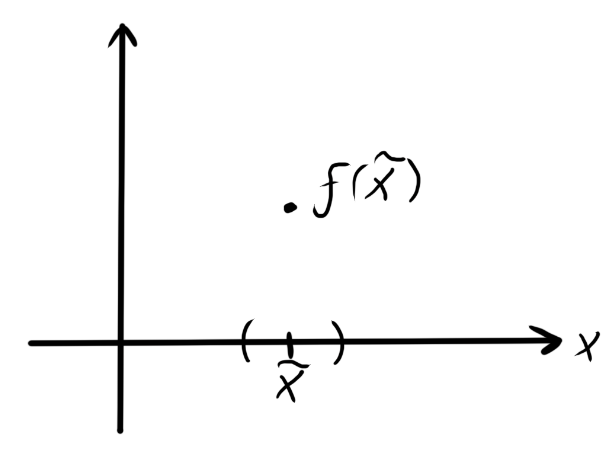
\includegraphics[width=0.5\textwidth]{/Users/vladbelousov/Desktop/Semestr_4-FP-NSU/ЭиО/Лекции_по_дням/image/8.png}
\end{center}

2) \(\displaystyle  \psi = \varphi +\frac{\pi}{2}    \) 

\[ \cos  ( kz - \omega t \varphi+ \frac{\pi}{2} )= \cos( kz - \omega t \varphi)\cos \frac{\pi}{2}-\sin( kz - \omega t \varphi)\sin  \frac{\pi}{2}   \] 

\[ \mathrm{Re}\vec{E }= |c_1|\vec{e_x}\cos ( kz - \omega t + \varphi)  - |c_2|\vec{e_y}\sin( kz - \omega t + \varphi)   \] 

3) \( \displaystyle \psi=\varphi - \frac{\pi}{2}  \) 

\[ \mathrm{Re}\vec{E }= |c_1|\vec{e_x}\cos ( kz - \omega t + \varphi)  + |c_2|\vec{e_y}\sin( kz - \omega t + \varphi)   \] 

\begin{center}
    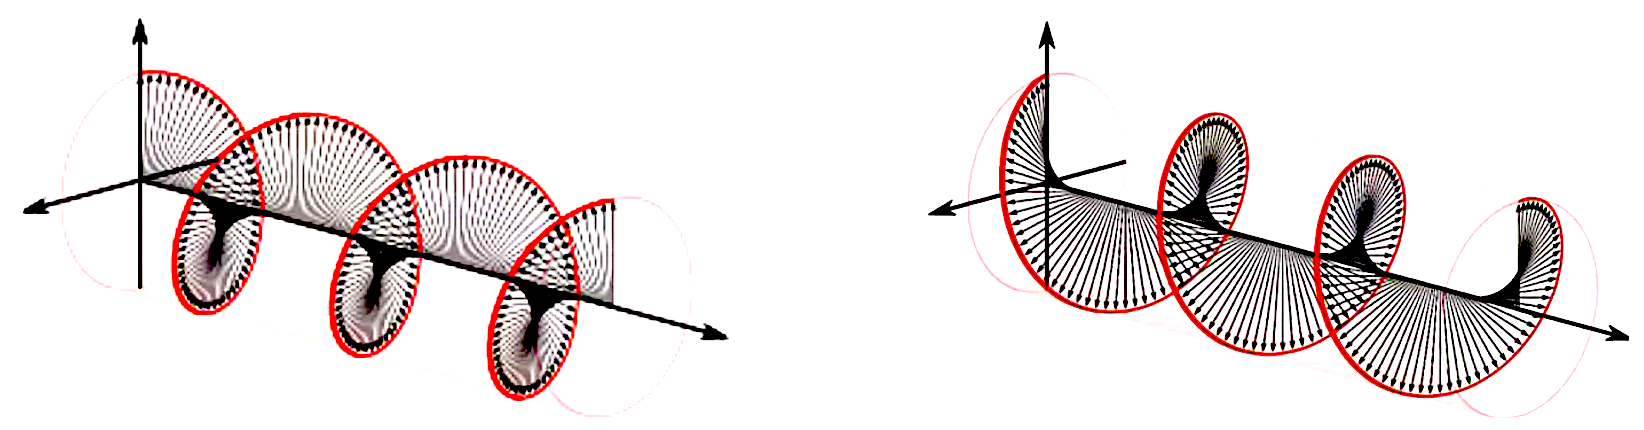
\includegraphics[width=0.8\textwidth]{/Users/vladbelousov/Desktop/Semestr_4-FP-NSU/ЭиО/Лекции_по_дням/image/9.png}
\end{center}


В случае произвольных  \( c_1, c_2 \)  эллипс повернут на некоторый угол относительно оси x (задача на семинаре).

\section{Средний по времени плотность  потока энергии в ПМВ}

\[ \vec{E_0}= c_1\vec{e_x}+ c_2 \vec{e_y} \] 

\[ \overline{\vec{S}} = \frac{c}{\sqrt{\varepsilon \mu}} \vec{n} \frac{\varepsilon\vec{E}}{4 \pi} = \frac{c}{\sqrt{\varepsilon \mu}} \vec{n} \frac{\varepsilon}{4 \pi} (\vec{E_x}+ \vec{E_y} )-\frac{c}{\sqrt{\varepsilon \mu}}\vec{n} \frac{\varepsilon}{4 \pi}( \frac{|c_1| ^2}{2}+ \frac{|c_2| ^2}{2} )  =  \] 

\[ = \frac{c}{\sqrt{\varepsilon \mu}} \vec{n} \frac{\varepsilon}{8 \pi} ( \vec{E_0}, \vec{E_0^*} )  \] 

\section{Фурье-преобразование электромагнитных полей}

Для периодической функции (\( f(t)= f(t+T) ,T\)) - период, можно использовать следующее представление: 

\[ f(t)= \frac{1}{\sqrt{T}} \sum_{n=- \infty }^{+ \infty }f_n e^{- i \omega nt } , \omega = \frac{2 \pi}{T}, f_n = \frac{1}{\sqrt{T}}  \int_{0}^{T}f(t)e^{+i \omega_0 nt} dt      \] 


Для непериодических функций Фурье представление в виде интеграла: 

\[ f(t)= \frac{1}{\sqrt{2 \pi}} \int_{-\infty }^{+\infty} \hat{f}e^{-i \omega t}d \omega, \hat{f}( \omega)= \frac{1}{\sqrt{2 \pi}} \int_{-\infty }^{+\infty}    f(t) e^{+i \omega t}dt     \] 

Для периодической функции: \( \hat{f}( \omega)= \frac{\sqrt{2\pi}}{\sqrt{T}} \sum ^{+\infty }_{n = - \infty } f_n \delta( \omega- n \omega_0)     \) 

\[ f(\lambda)= \frac{1}{\sqrt{2 \pi}}\int _{-\infty }^{+\infty} \hat{f}(k)e^{i k x }d k  , \hat{f}(k)= \frac{1}{\sqrt{2 \pi}} \int_{-\infty}^{\infty} f(x)e^{- ikx} dx    \] 

Напоминание про свойства \( \delta \) - функции

\[ I(t)= \int_{-\infty}^{\infty} e^{- i \omega t} d \omega = \lim_{\Omega \to \infty} \int_{-\Omega}^{\Omega}e^{- i \omega t} d \omega  = \lim \frac{-e^{-i \Omega t} + e^{i \Omega t}}{it 2 \Omega}  2 \Omega = \lim_{\Omega \to \infty}   2 \Omega  \cdot\mathrm{sinc}(\Omega t)    \] 

\begin{center}
    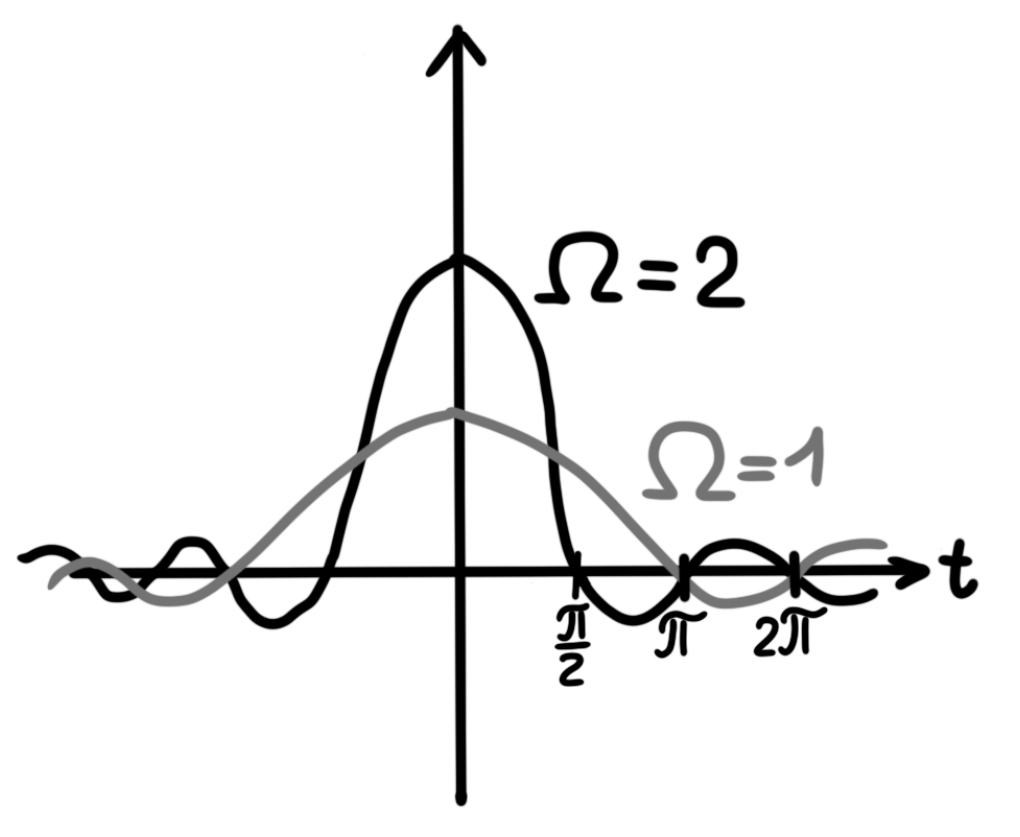
\includegraphics[width=0.4\textwidth]{/Users/vladbelousov/Desktop/Semestr_4-FP-NSU/ЭиО/Лекции_по_дням/image/10.png}
\end{center}

\[ \int_{-\infty }^{\infty} I (t)dt =\lim \int_{-\infty}^{\infty} 2 \Omega \frac{\sin  ( \Omega t)}{\Omega t}dt = 2 \int_{- \infty }^{\infty} \frac{ \sin x}{x}dx = 2 \cdot \mathrm{Im} \left[ \int_{-\infty }^{\infty} \frac{e^{ix} }{x} dx \right]      \] 

\[ \int_{C} \frac{e^{ix} }{x} dx =0 = \underbrace{\int_{|z|= R}}_{=0}  + \int_{-\infty}^{-\rho} + \int_{|z|= \rho} + \int_{ \rho}^{\infty}       \] 

\[ \int_{-\infty}^{\infty} \frac{e^{ix} }{x} dx = - \int_{|z|=\rho} \frac{e^{i \rho e ^{i \varphi} } \cdot \rho i e^{ i \varphi} d \varphi }{\rho e^{i \varphi}} =- i \int_{\pi}^{0} d \varphi= i \pi \Rightarrow \int_{-\infty }^{\infty} I ( t)dt = 2\pi      \] 

\[ \int_{-\infty }^{\infty}  e^{- i \omega t} d \omega = 2 \pi \delta ( t) \quad \int_{-\infty}^{\infty} e ^{ - i \omega t }dt = 2 \pi \delta(\omega)  \]

\[ \int_{-\infty}^{\infty}   e^{- i \omega( t - \tau)} d \omega = 2 \pi \delta ( t - \tau )\quad  \int_{-\infty}^{\infty}    e^{-i (\omega- \omega ') t} d \omega = 2 \pi \delta ( \omega- \omega' )   \] 

1)\[  \delta ( t- \tau )= \frac{1}{ \sqrt{ 2 \pi }} \int_{-\infty}^{  \infty} \underbrace{\frac{1}{ \sqrt{2\pi }} e^{+i \omega t} }_{\delta ( t - \tau) }e^{- i \omega t} d \omega \] 

2)\[ f(t)= \int_{-\infty}^{\infty} f(\tau ) \delta ( t - \tau)d \tau = \int_{-\infty}^{\infty} \frac{f(\tau)d \tau}{2 \pi} \int_{-\infty}^{\infty} e^{- i \omega ( t - \tau ) }d \omega = \frac{1}{ \sqrt{2 \pi}} d \omega e ^{- \omega t } \frac{1}{\sqrt{2 \pi}} \int_{-\infty}^{\infty} d \tau f( \tau) e^{i \omega \tau}       \] 

3) \[ \int_{-\infty}^{\infty}   f_1 ( t)f_2 ^{*}dt  = \int_{-\infty}^{\infty}   dt \frac{1}{\sqrt{2\pi}}\int_{-\infty}^{\infty} \hat{f_1 }(\omega)e ^{-i \omega t} d \omega \frac{1}{\sqrt{2 \pi}} \int _{-\infty}^{\infty} \hat{f_2 }(\omega') e^{i \omega' t} d \omega'    = \]

\[ = \int_{-\infty}^{\infty}    \hat{f_1} (\omega)d \omega \hat{f_2 ^{*} }(\omega') d \omega' \frac{1}{2 \pi} 2\pi \delta ( \omega -\omega') f_1(t)= \int_{-\infty }^{\infty}\hat{f_1 }(\omega) \hat{f_2 ^{*} }(\omega) d \omega  \]

\[ \Rightarrow \int_{-\infty}^{\infty} |f(t)| ^2 dt = \int  _{-\infty}^{\infty} |\hat{f}(\omega)| ^2 d \omega - \text{ равенство Парсеваля }   \] 

\begin{center}
    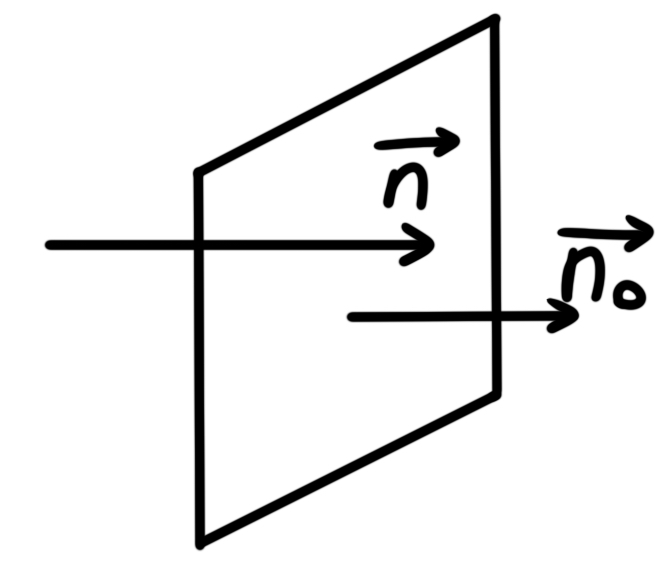
\includegraphics[width=0.2\textwidth]{/Users/vladbelousov/Desktop/Semestr_4-FP-NSU/ЭиО/Лекции_по_дням/image/12.png}
\end{center}

Прошедшая энергия за \( \infty \)  интервал времени через см\( ^2 \)

\[ = \int (\vec{S}\vec{n})dt= \frac{c}{\sqrt{\mu \varepsilon}} \frac{\varepsilon}{ 4\pi }  \int_{-\infty}^{\infty} \vec{E} ^2(t)dt = \frac{c}{\sqrt{\mu \varepsilon}} ( \vec{n}\vec{n_0}) \frac{\varepsilon}{4 \pi} \int_{-\infty}^{\infty} |\hat{\vec{E}}(\omega) | ^2 d \omega  \] 

Свойства Фурье-преобразования: 

1) Пусть \( \displaystyle f(t) \in  \mathbb{R} \Rightarrow f(t)= f^*(t)= \frac{1}{\sqrt{2\pi}}\int_{-\infty}^{\infty} \hat{f^{*} }e ^{+i \omega t} d \omega =[\omega \to  - \omega ']   =  \)

\[ =\frac{1}{\sqrt{ 2 \pi }}(- )\int_{-\infty}^{\infty} d \omega ' \hat{f^{*} } ( -\omega ')e^{- i \omega' t}     \] 

\[ \hat{f^*} (- \omega) = \hat{f}(\omega)  \]

\[ \hat{f^*} ( \omega) = \hat{f}(-\omega) \] 


2) Спектр сдвинутого по времени сигнала:

\begin{center}
    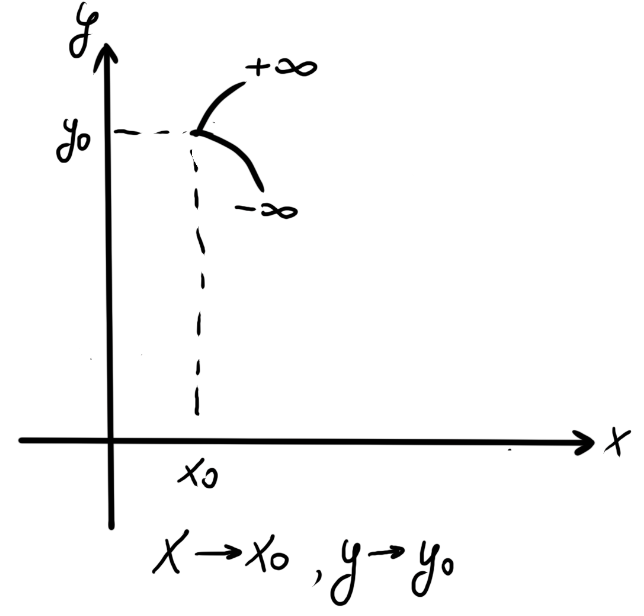
\includegraphics[width=0.5\textwidth]{/Users/vladbelousov/Desktop/Semestr_4-FP-NSU/ЭиО/Лекции_по_дням/image/11.png}
\end{center}
\[  \hat{F}(\omega)=\frac{1}{\sqrt{2 \pi}}\int_{-\infty}^{\infty} f(t- T)e^{+ i \omega t }dt = \frac{1}{\sqrt{2\pi}} \int_{-\infty}^{\infty} f(t' )e^{+ i \omega t } e^{i \omega T} dt =\hat{f}(\omega)e^{i \omega T}         \]  

3) \[  F( t)= f(t) e^{- i \omega_0 t  }\quad  F(\omega)= \frac{1}{\sqrt{2 \pi}} \int_{-\infty}^{\infty}   f(t) e ^{- i \omega_0 t} e ^{i \omega t}dt  = \hat{f}( \omega - \omega_0) \]  

\begin{center}
    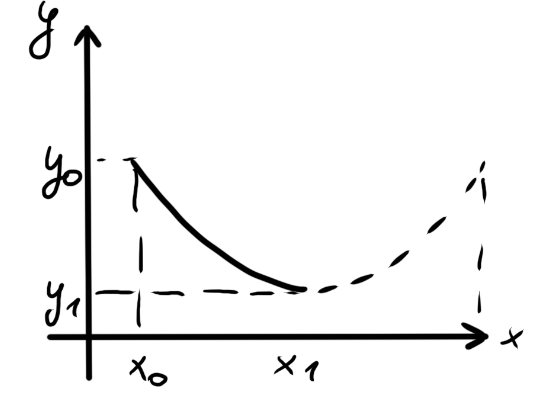
\includegraphics[width=0.5\textwidth]{/Users/vladbelousov/Desktop/Semestr_4-FP-NSU/ЭиО/Лекции_по_дням/image/13.png}
\end{center}

4) Спектр N повторенного сигнала: 

\[ F(t)= \sum_{n=0}^{N-1} f( t - nT); \quad F(\omega)= \sum _{n=0}^{N-1} \hat{f}(\omega) e^{i \omega n T} = f( \omega ) \frac{ e ^{i \omega NT} -1}{e ^{i \omega T} -1}  = \hat{f} ( \omega )= \hat{f}(\omega) e^{i \omega T \frac{ N-1 }{2} } \boxed{\frac{\sin \left( \frac{\omega T}{2}N  \right) }{\sin \left( \frac{\omega T}{2} \right)}}   \]

Последний выделенный  множитель в правой части уравнения - это интерференционный множитель.

\begin{center}
    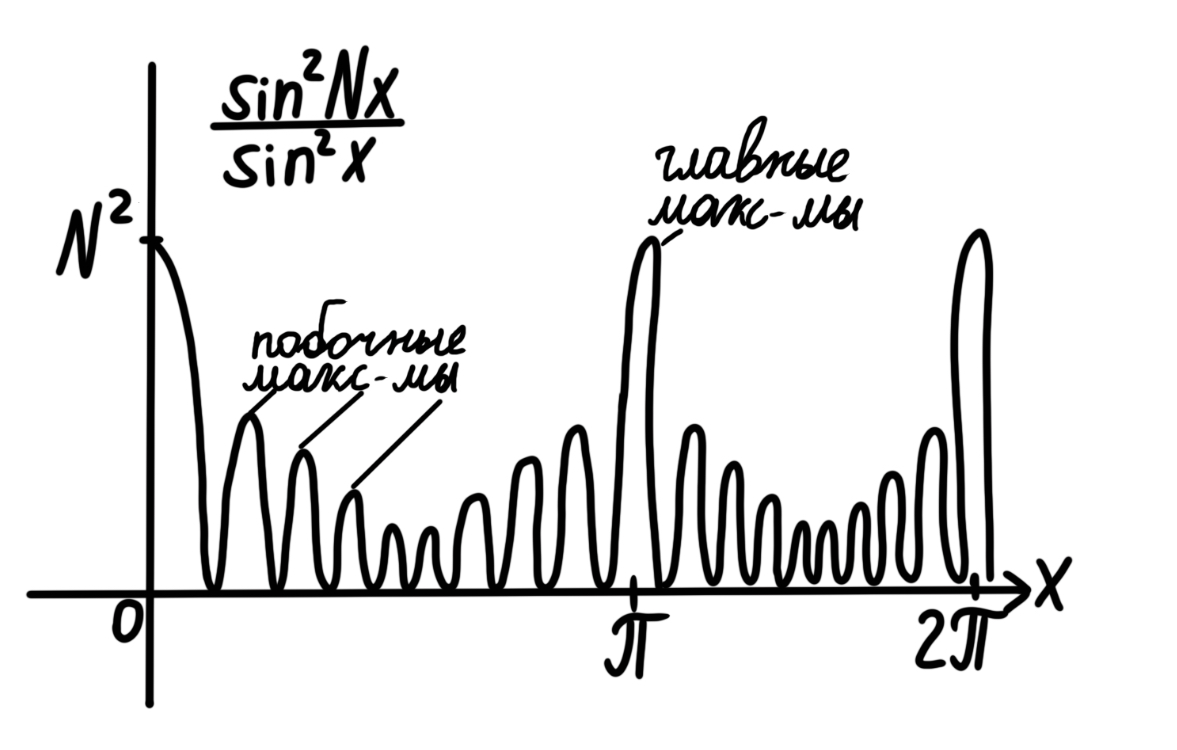
\includegraphics[width=0.5\textwidth]{/Users/vladbelousov/Desktop/Semestr_4-FP-NSU/ЭиО/Лекции_по_дням/image/14.png}
\end{center}
\[ x=  m \pi \varepsilon, \varepsilon > 0  \] 

\[ \frac{\sin ^2 (N ( m\pi+ \varepsilon))}{\sin  ^2 ( m \pi + \varepsilon )} = N ^2   \] 
%%-------------------------------%%


% Закрытие документа, если файл компилируется отдельно
\ifdefined\mainfile
    % Если это основной файл, не нужно заканчивать документ
\else
    \end{document}
\fi
% Условная компиляция для самостоятельной работы
\ifdefined\mainfile
    % Если это часть основного файла, не добавляем начало и конец документа
\else
    \documentclass[12pt, a4paper]{report}
    \usepackage{/Users/vladbelousov/Desktop/Semestr_4-FP-NSU/Настройка/library}
    \usepackage[utf8]{inputenc} % Подключение поддержки UTF-8
    \begin{document}
\fi

%%-------------------------------%%

\section{Продолжение. Спектр свертки двух функций}

\[ F(t)= \int_{-\infty}^{\infty} f(\tau)g(t- \tau)d \tau= \int_{-\infty}^{\infty} d \tau \frac{1}{\sqrt{2 \pi}} \int_{-\infty}^{\infty} \hat{f} (\omega) e ^{- i \omega \tau} d \omega \frac{1}{\sqrt{2\pi}} \int_{-\infty}^{\infty} \hat{g} (\omega') e^{i \omega' (t - \tau)} d \omega'     =\] 

\[ =\int_{-\infty}^{\infty}  d \omega \int_{-\infty}^{\infty} d \omega ' \hat{f} (\omega) \hat{g}(\omega ') e^{- \omega ' t } \frac{1}{2 \pi } \int_{-\infty}^{\infty} \underbrace{d \tau e^{- i (\omega - \omega ' )\tau}}_{=2\pi \delta(\omega- \omega')} = \int_{-\infty}^{\infty}  d \omega \hat{f} ( \omega) \int_{-\infty}^{\infty}  d \omega ' \hat{g} ( \omega ' ) \delta(\omega - \omega ') e ^{-i \omega' t} =        \] 

\[ = \frac{1}{\sqrt{2 \pi}} \int_{-\infty}^{\infty}  \sqrt{ 2 \pi} \hat{f}( \omega ) \hat{g} (\omega   )e ^{- i\omega t}   d \omega \Rightarrow F(t) \risingdotseq \sqrt{ 2 \pi } \hat{f}( \omega ) \hat{g } ( \omega)  \] 

\section{Соотношение неопределенностей}

\begin{definition}
    Определенная связь между длительностью сигнала и шириной его спектра называется соотношение неопределенностей.
\end{definition}

Покажем эту связь на примерах: 

1) Спектр прямоугольного сигнала \( E_1 (t) =\begin{cases}
E_0 , |t| \le  \frac{\tau}{2} \\
0 , |t| > \frac{\tau}{2}
\end{cases} \) E(t) - сигнал.

\begin{center}
    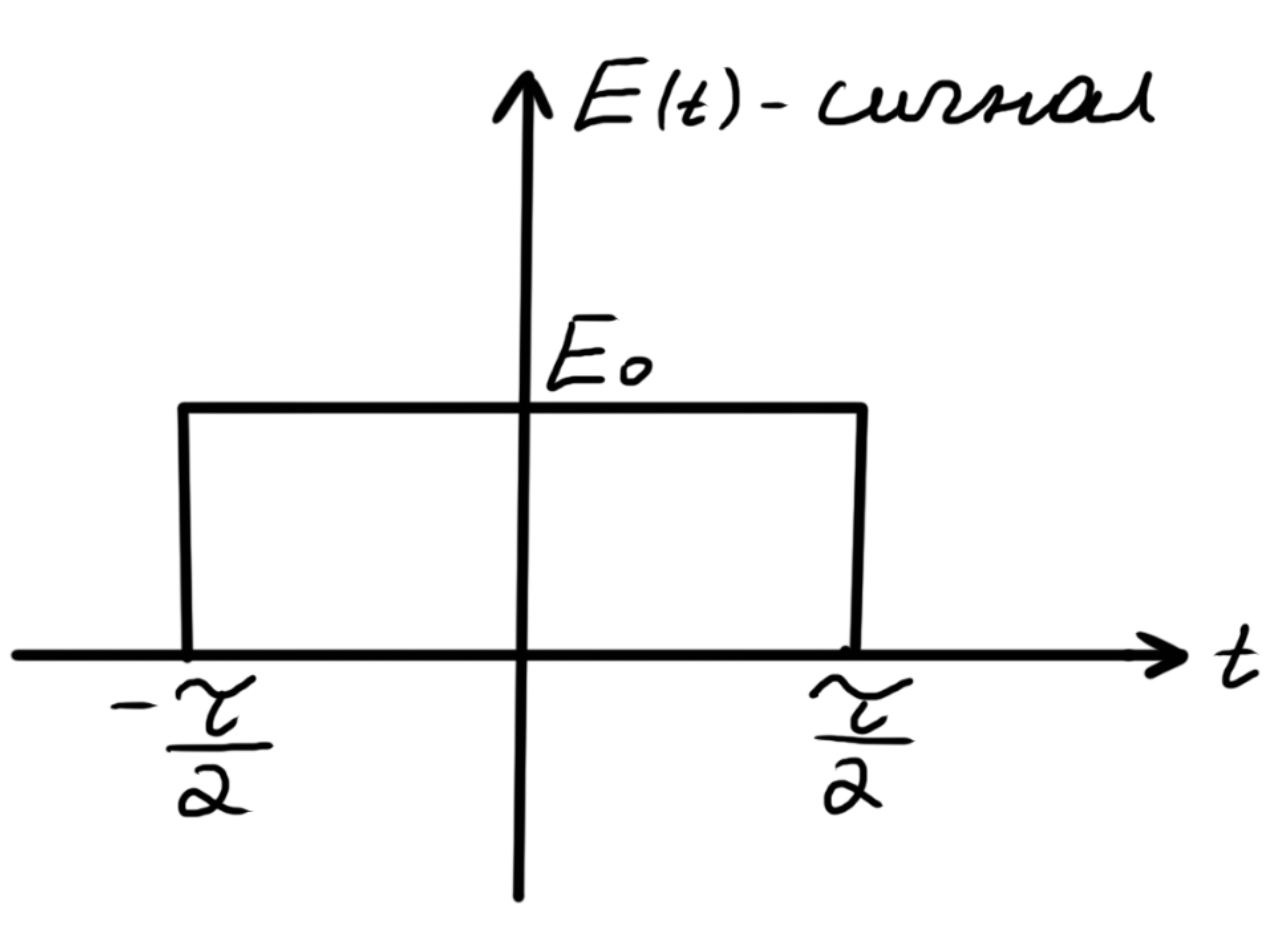
\includegraphics[width=0.3\textwidth]{/Users/vladbelousov/Desktop/Semestr_4-FP-NSU/ЭиО/Лекции_по_дням/image/15.png}
\end{center}

\[ \hat{E}(\omega)= \frac{1}{\sqrt{2 \pi}} \int_{\frac{\tau}{2} }^{-\frac{\tau}{2} } E_0 E^{+ i \omega t} d t = \frac{E_0 \tau}{\sqrt{2 \pi}} \frac{e^{ i \omega \frac{\tau}{2} }- e^{ - i \omega \frac{\tau}{2} }}  {2 i \omega \frac{\tau}{2} }     = \frac{E_0 \tau}{\sqrt{2 \pi}} \mathrm{sinc} ( \frac{\omega \tau}{2} )   \] 

\begin{center}
    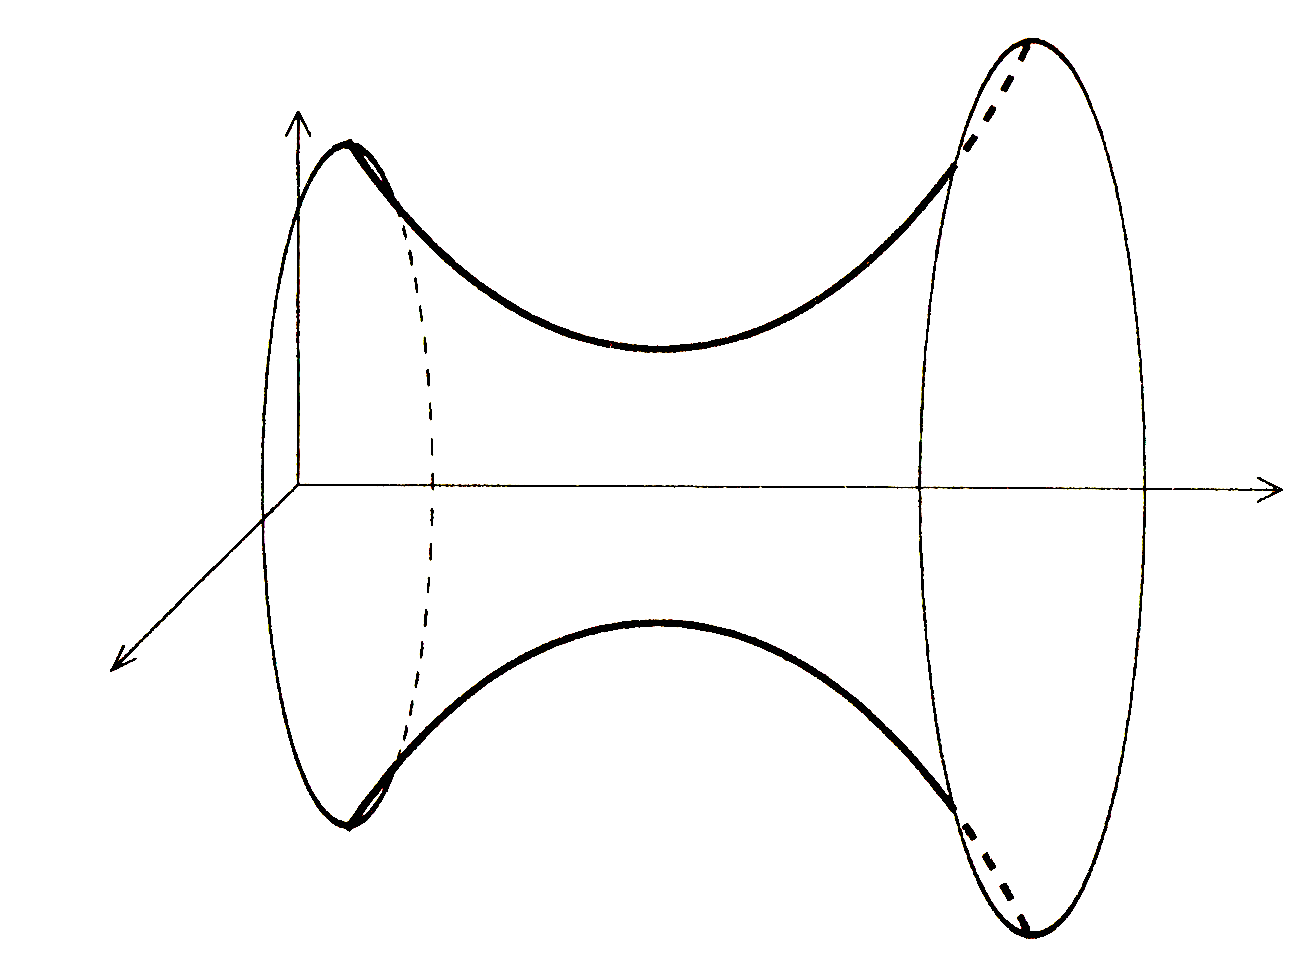
\includegraphics[width=0.5\textwidth]{/Users/vladbelousov/Desktop/Semestr_4-FP-NSU/ЭиО/Лекции_по_дням/image/16.png}
\end{center}

Спектральная плотность энергии = \( |\hat{E } (\omega)| ^2  \) 

\begin{center}
    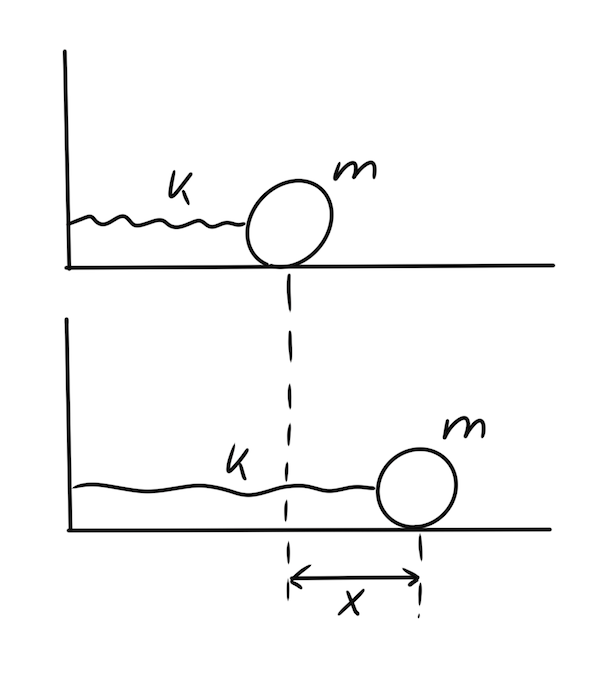
\includegraphics[width=0.5\textwidth]{/Users/vladbelousov/Desktop/Semestr_4-FP-NSU/ЭиО/Лекции_по_дням/image/17.png}
\end{center}

\[ \Delta \omega \sim  \frac{2 \pi}{ \tau} \Rightarrow \Delta \omega \tau \sim \pi - \text{ соотношение неопределенности}     \] 

\[ \tau \to  \infty \Rightarrow \hat{E } \sim  \delta ( \omega)  \] 



2)Спектр синусоидальной волны: 

\[ \begin{aligned}
    E_2 ( t) = \begin{cases}
        E_0 \sin  \omega_0 t , |t| \le \frac{\tau}{2} \\
        0 , |t| > \frac{\tau}{2}
    \end{cases}, 
    \omega_0 = \frac{2 \pi}{\tau} \quad \text{, пусть } \tau= N T , N(\text{целое} ) \gg 1 
\end{aligned} \] 

\begin{center}
    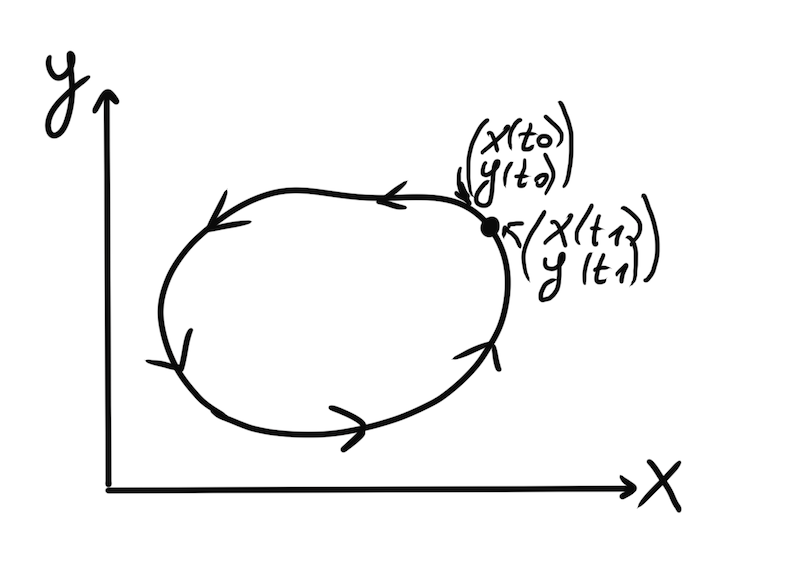
\includegraphics[width=0.5\textwidth]{/Users/vladbelousov/Desktop/Semestr_4-FP-NSU/ЭиО/Лекции_по_дням/image/18.png}
\end{center}


\[ \hat{E_2 } ( \omega) = \frac{1}{ \sqrt{2 \pi}} \int_{-\infty}^{\infty} \frac{ e^{ i \omega_0 t } - e^{- i \omega_0 t} }{2 i} e^{i \omega t} dt  = \frac{1}{2i} \left\{ \frac{E_0 \tau}{\sqrt{2 \pi}}\mathrm{sinc} \left[ (\omega + \omega_0) \frac{\tau}{2}  \right] -    \frac{E_0 \tau}{\sqrt{2 \pi}}\mathrm{sinc} \left[ (\omega - \omega_0) \frac{\tau}{2}  \right]\right\}      \] 

\begin{center}
    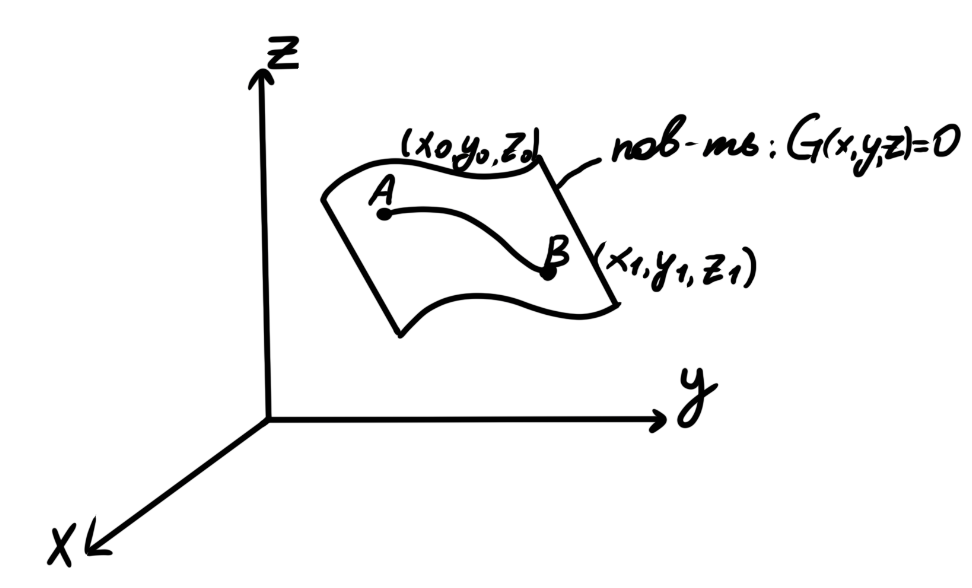
\includegraphics[width=0.45\textwidth]{/Users/vladbelousov/Desktop/Semestr_4-FP-NSU/ЭиО/Лекции_по_дням/image/19.png}
    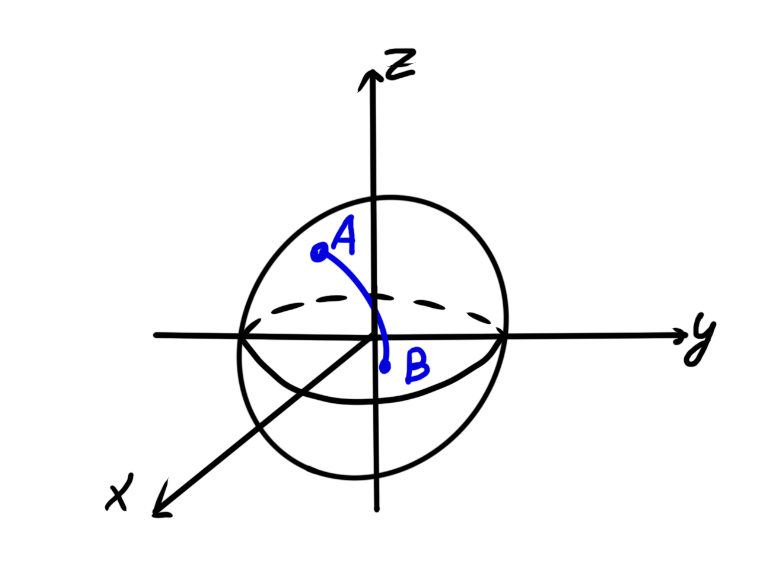
\includegraphics[width=0.45\textwidth]{/Users/vladbelousov/Desktop/Semestr_4-FP-NSU/ЭиО/Лекции_по_дням/image/20.png}
\end{center}

Если \( \frac{\Delta \omega}{\omega_0} \ll 1   \), то такая волна - квазимонохроматическая. 

3) Спектр радиационно затухающего осциллятора:

Механистическая модель атома:

\[ E(t)= \begin{cases}
E_0 e^{ \gamma t} \cos \omega_0 t , t >0\\
0, t < 0
\end{cases} \] 

\[ \gamma = \frac{e ^2 \omega_0 ^2 }{3 m c ^2 } \sim 10 ^9 c^{-1} \quad  \omega_0 \approx 2 \cdot 10^{16} \frac{rad}{c}  \Rightarrow f \sim 3 \cdot 10^8 c^{-1}    \] 

\[ e^{ - \gamma t} = e^{- \frac{t}{\tau} } \Rightarrow \tau \sim \frac{1}{\gamma}      \] 

\begin{center}
    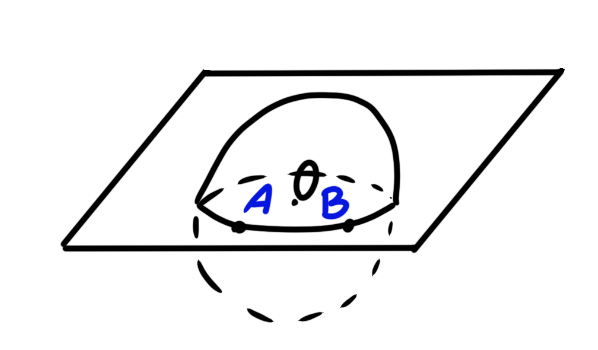
\includegraphics[width=0.5\textwidth]{/Users/vladbelousov/Desktop/Semestr_4-FP-NSU/ЭиО/Лекции_по_дням/image/21.png}
\end{center}

\[ \hat{E} ( \omega ) =\frac{1}{\sqrt{2 \pi}}  \int_{0}^{\infty} E_0 e^{ - \gamma t } \frac{ e^{i \omega_0 t}+ e^{- i \omega_0 t} }{2}  e^{+ i \omega t }   d t     \] 

\[ \hat{E}(\omega) = \frac{E_0}{2 \sqrt{2 \pi}} \left\{ -\frac{1}{- \gamma + i (\omega + \omega_0)}-\frac{1}{- \gamma + i (\omega - \omega_0)}  \right\} = \hat{ f}( \omega + \omega_0) \hat{f}( \omega - \omega_0 )  \]

\[ \lvert \hat{f}(\omega- \omega_0 )   \rvert ^2 = \frac{E_0 ^2 }{8 \pi} \] 

\begin{center}
    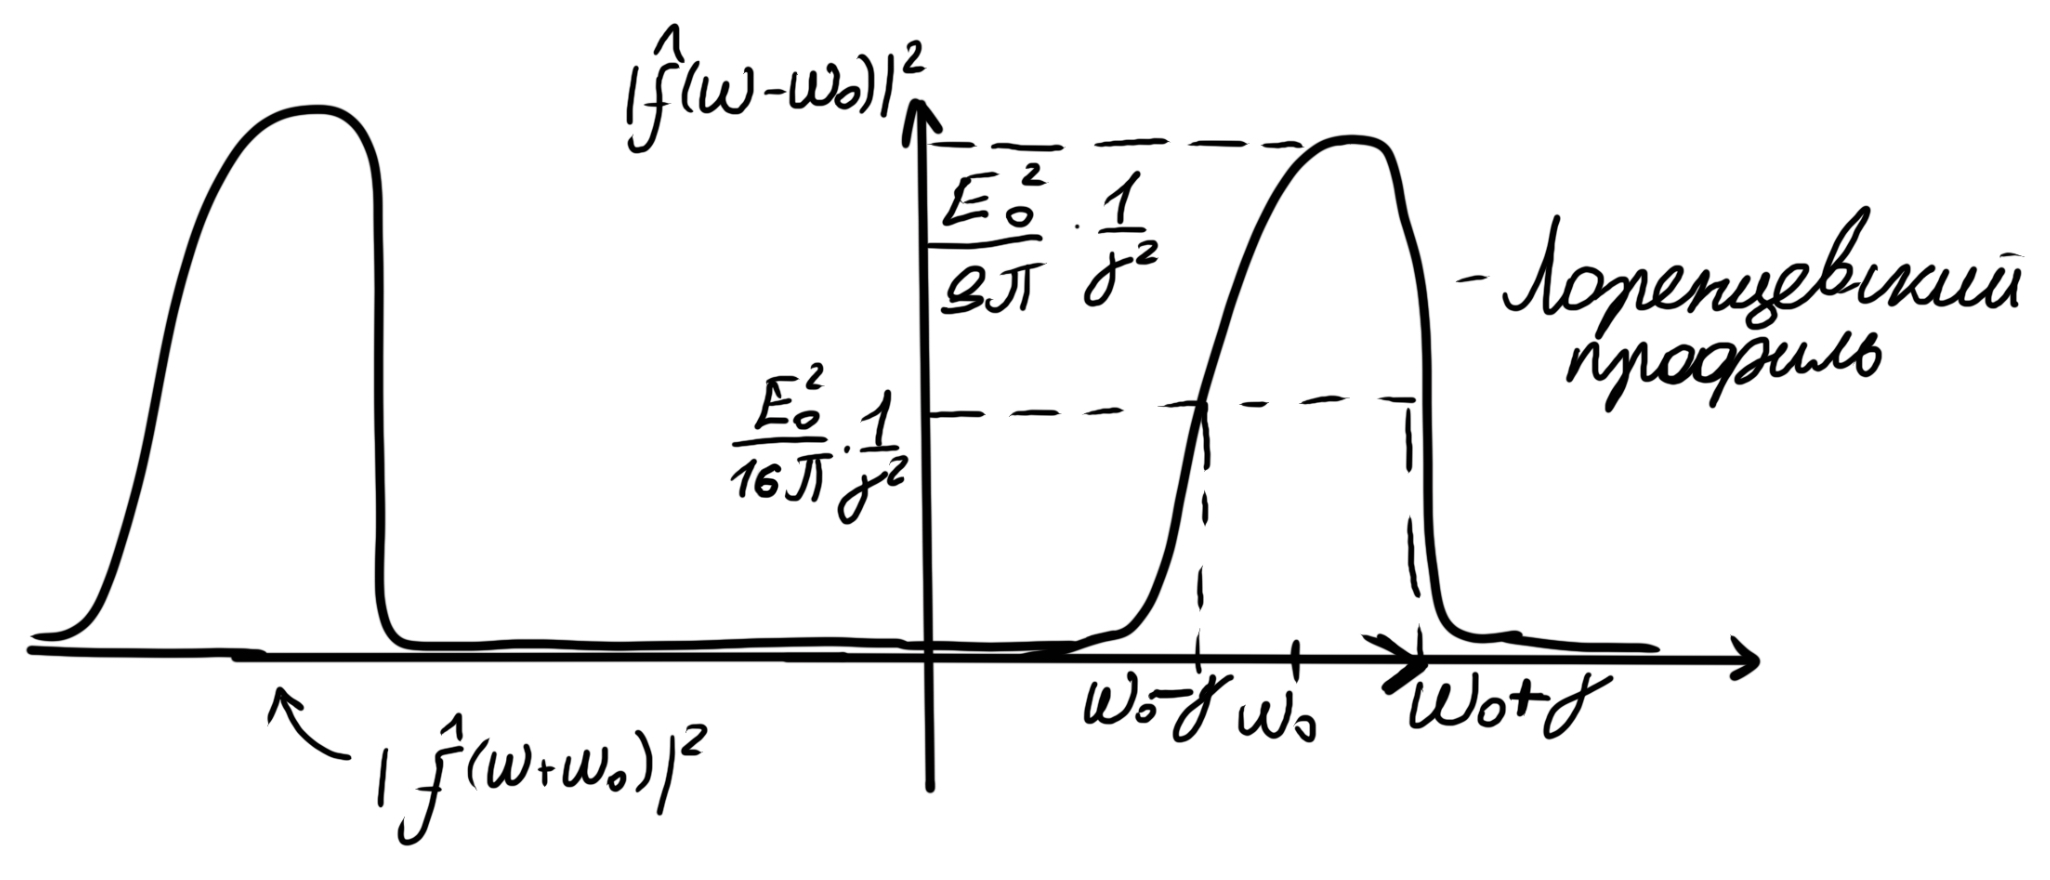
\includegraphics[width=0.55\textwidth]{/Users/vladbelousov/Desktop/Semestr_4-FP-NSU/ЭиО/Лекции_по_дням/image/22.png}
\end{center}

\[ \Delta \omega \sim  2 \gamma - \text{ширина спектра}  \] 

\[ \Delta \omega \underbrace{\Delta t}_{\sim  \tau}  \sim 2 \gamma \frac{1}{\gamma} \sim 2   \] 

\[ |\hat{E} ( \omega ) | ^2 = |\hat{f}(\omega + \omega_0) | ^2 + |\hat{f}(\omega - \omega_0) | ^2 + \cancel{\text{поправка}}  \] 

Поправка  мала, если \( 10^9 c^{-1} \sim\Delta \omega \ll \omega_0 \sim 2 \cdot 10^{16} \frac{rad}{c}  \) 

4) Спектр гауссовой функции : \( f(x) = E_0 e^{ -\alpha x ^2} \quad  \hat{f}( x) = \frac{1}{\sqrt{2 \pi}} \int_{-\infty}^{\infty}   f( x) e^{- i kx }dx =     \) 

\[ \frac{1}{\sqrt{2 \pi}}E_0 \int_{-\infty}^{\infty} e^{- \alpha x ^2 - ikx } dx ; -\alpha x ^2 - ikx = -\alpha \left( x ^2 + 2x \frac{ik}{2 \alpha} - \frac{k ^2}{4 \alpha ^2}   \right) - \frac{k ^2}{4\alpha} =  - \alpha \left( x + \frac{ik}{2\alpha} \right) ^2 - \frac{k ^2}{4\alpha}    \] 

\begin{center}
    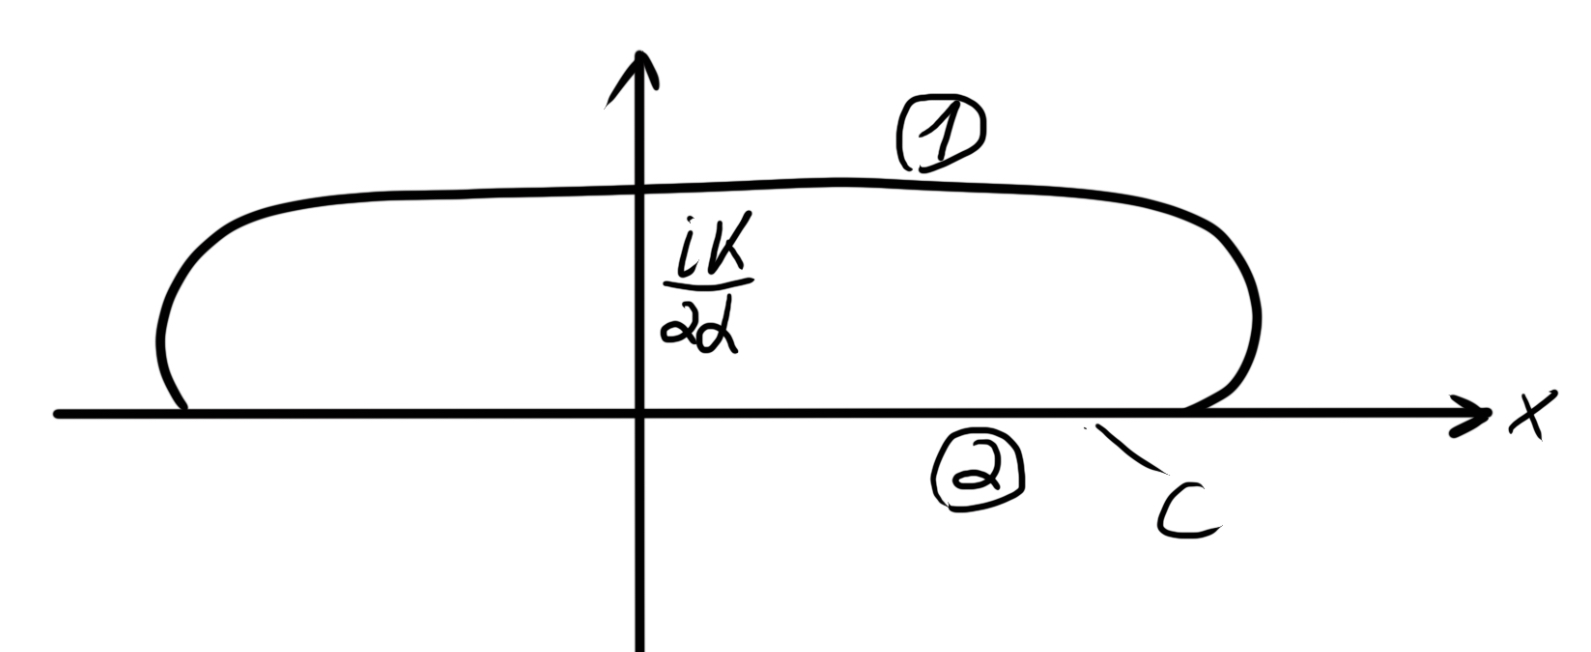
\includegraphics[width=0.4\textwidth]{/Users/vladbelousov/Desktop/Semestr_4-FP-NSU/ЭиО/Лекции_по_дням/image/23.png}
\end{center}

\[  \int_{C} e^{- \alpha z ^2 }dz = 0 = \int_{1} + \int_{ 2} \Rightarrow \int_{1} = \int _{-2}  \] 

\[ \int_{-\infty}^{\infty} e^{-\alpha z ^2 } dz = \int_{-\infty}^{\infty} e^{ - \alpha x ^2 } dx = \sqrt{\frac{\pi}{\alpha} }    \] 

\[ \hat{f} (k) = \frac{ E_0}{\sqrt{2 \pi}} \sqrt{\frac{\pi}{\alpha}} e^{- \frac{k ^2}{4 \alpha} }    \]

\begin{center}
    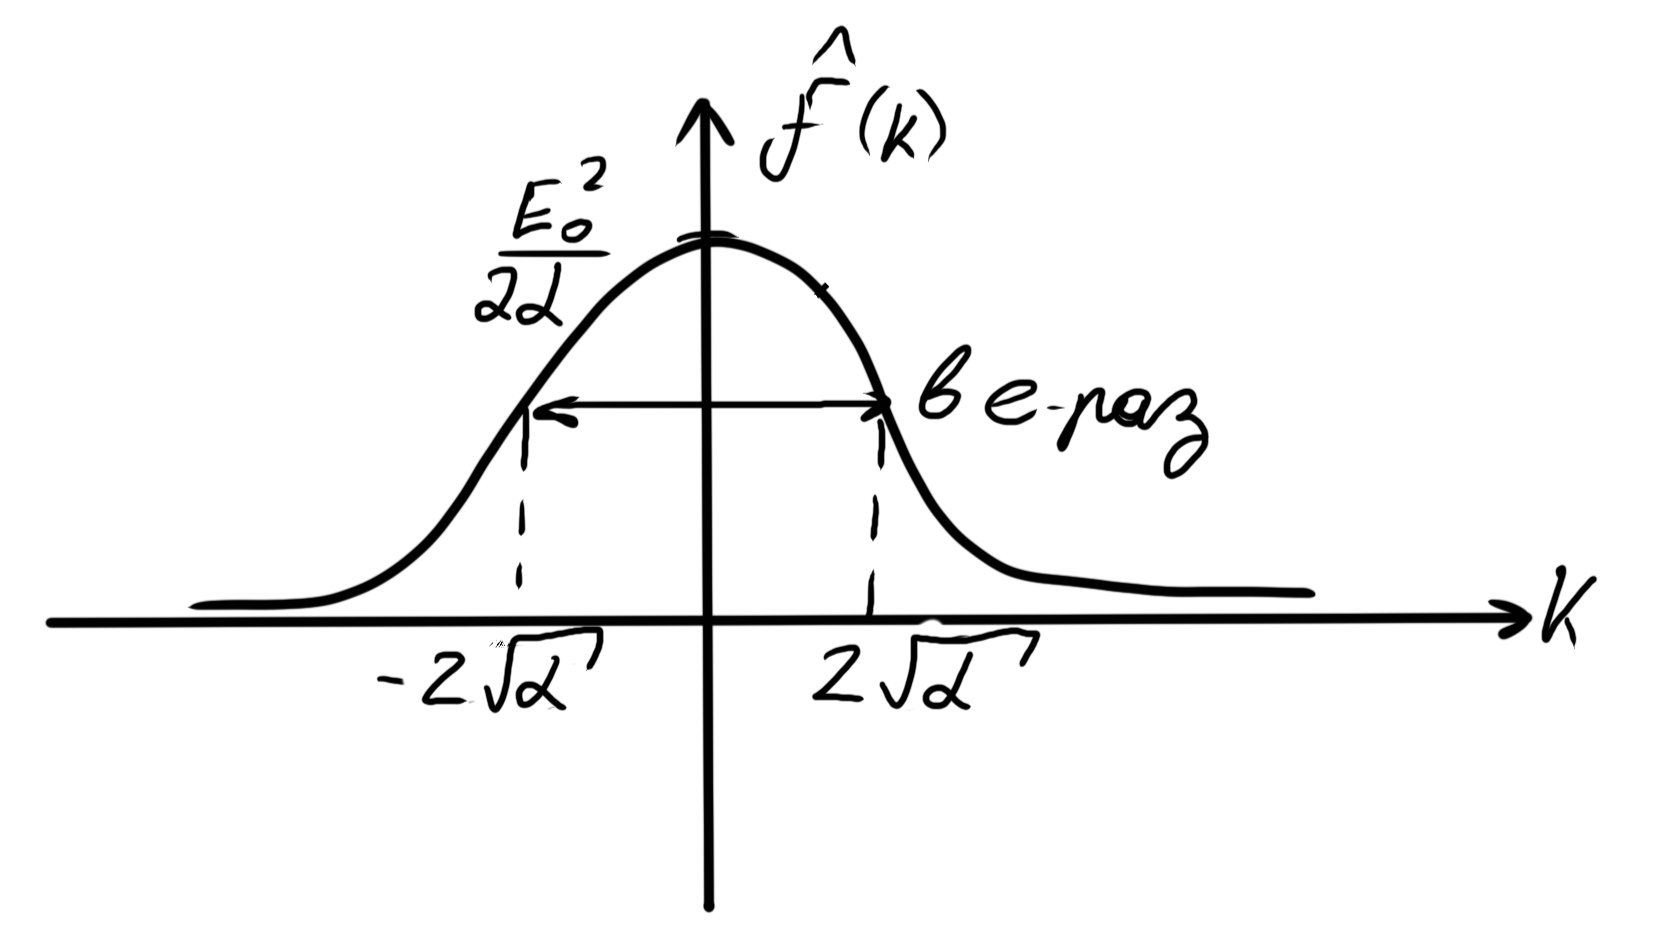
\includegraphics[width=0.45\textwidth]{/Users/vladbelousov/Desktop/Semestr_4-FP-NSU/ЭиО/Лекции_по_дням/image/24.png}
    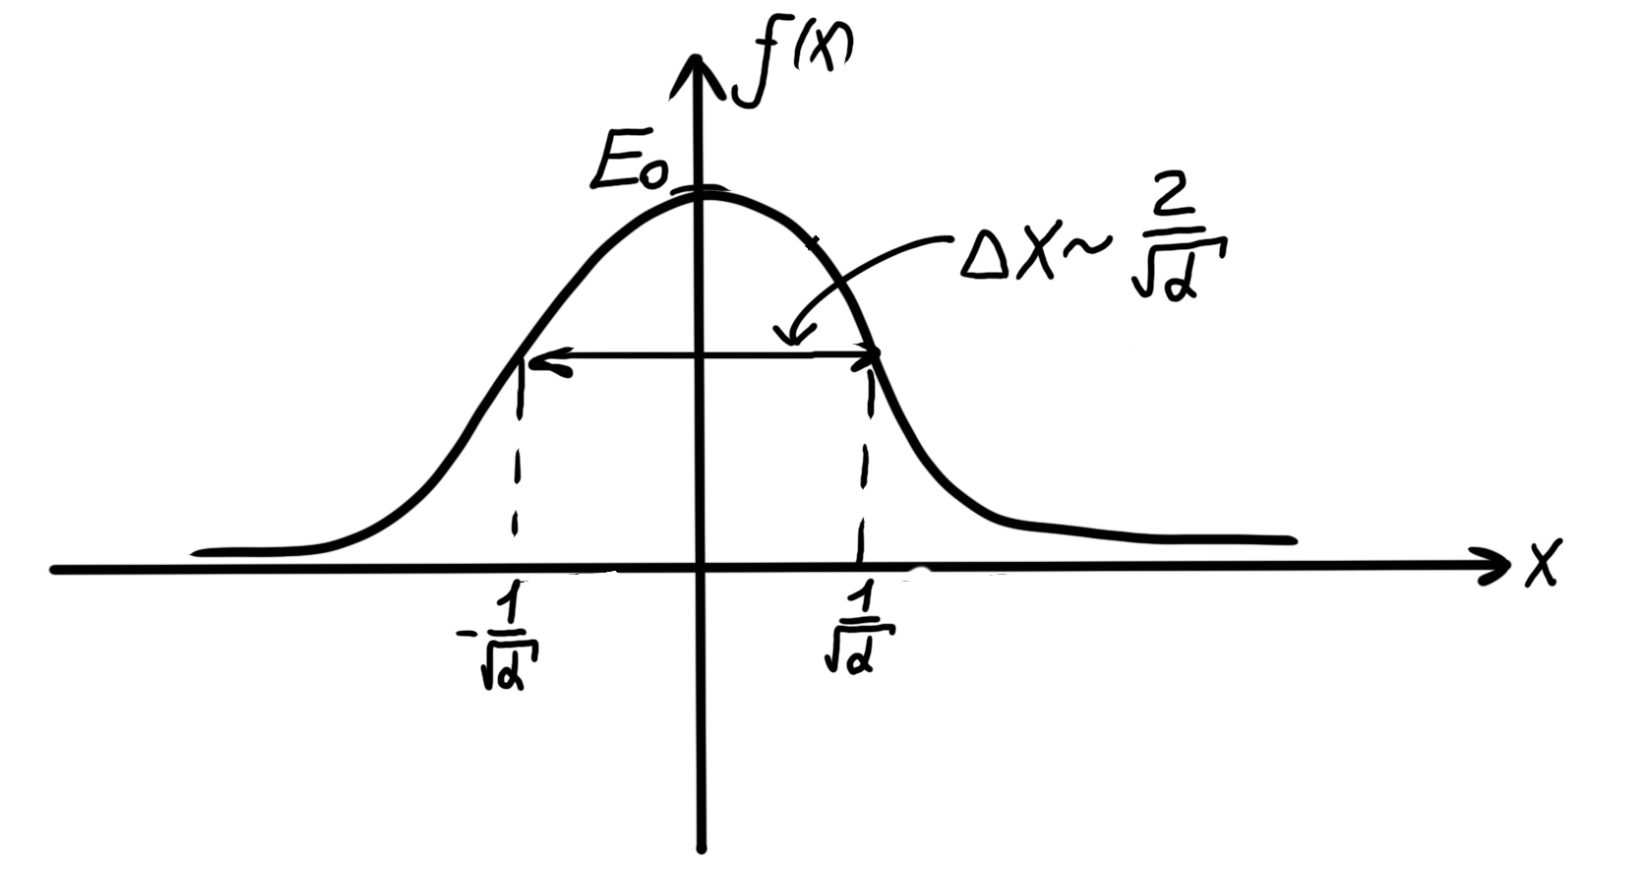
\includegraphics[width=0.45\textwidth]{/Users/vladbelousov/Desktop/Semestr_4-FP-NSU/ЭиО/Лекции_по_дням/image/25.png}
\end{center}


\[\begin{aligned}
    \begin{array}{l}
        \Delta k \sim  4 \sqrt{\alpha} \\
        \Delta x \sim \frac{2}{\sqrt{\alpha}}
    \end{array}
    \Rightarrow 
    \Delta k \Delta x \sim 8 \sim \pi 
\end{aligned} \] 

5) Модулированный гауссиан: \( E(x) = E_0 e^{ - \alpha x ^2} \cos k_0x \) 

\section{Преобразование Фурье функции четырех переменных (x,y,z,t). Уравнения Максвелла в Фурье преобразованиия}

\[ f(x,y,z,t) = \frac{1}{\sqrt{ 2 \pi} ^4} \iiiint \hat{f}(k_x,k_y,k_z,k_t) e^{  i k_x x } e^{ i k_y y } e^{  i k_z z } e^{ - i \omega t } dk_x dk_y dk_z dk_t    \] 

\[ f( \vec{r},t) = \frac{1}{(2 \pi) ^2 } \iiiint \hat{f} ( \vec{k}, \omega) e^{ i( \vec{k},\vec{r})- i\omega t} d^3 k d \omega    \]  

\[ \frac{\partial f( \vec{r},t)}{\partial t} = \frac{1}{( 2 \pi ) ^2} \iiiint \hat{f}(\vec{k}, \omega) ( - i \omega) e^{i \vec{k}\vec{r} - i \omega t} d^3 k d \omega \quad \frac{\partial f}{\partial t}  \risingdotseq   - i \omega \hat{f}( \vec{k}, \omega)    \] 

\[ \frac{\partial f (\vec{r},t)}{\partial x} \risingdotseq i k_x \hat{f}( \vec{k}, \omega) \]

\[ \mathrm{div} \hat{\vec{D}}(\vec{r},t) = \frac{\partial \hat{\vec{D_x}}}{\partial x} + \frac{\partial \hat{\vec{D_y}}}{\partial y} + \frac{\partial \hat{\vec{D_z}}}{\partial z} \risingdotseq i k_x \hat{D_x}(\vec{k}, \omega) + i k_y \hat{D_y}(\vec{k}, \omega) + i k_z \hat{D_z}(\vec{k}, \omega)  = i (\vec{k},\hat{\vec{D}}(\vec{r}, \omega) ) \] 

\[ \mathrm{rot}\hat{\vec{E}}  = [\nabla \times  \hat{\vec{E}} ] = \frac{1}{( 2 \pi ) ^2 } \iiiint \underbrace{\left[ (\nabla \times  \hat{\vec{E}} (\vec{k}, \omega)e^{i (\vec{k}\vec{r}) }   ) \right]}_{\nabla e^{i (\vec{k }, \vec{r })}   \times \vec{E } (\vec{k },\omega) }   e^{- i \omega t } d ^3 d \omega  =      \] 

\begin{center}
    Где \(\nabla e^{i (\vec{k }, \vec{r })} = \vec{e_x }i k_xe^{(i (\vec{k }, \vec{r }))}+ \vec{e_y } i k_y e^{(i (\vec{k }, \vec{r }))} + \vec{e_z } i k_z e^{(i (\vec{k }, \vec{r }))}= i\vec{k } e ^{ i ( \vec{k } , \vec{r})} \)    
\end{center}


\[= \frac{1}{( 2 \pi) ^2 } \iiiint \left[ i \vec{k} \times  \hat{\vec{E }}( \vec{k }, \omega)  \right] e^{i(\vec{k}, \vec{r})- i \omega t} d ^3 k d \omega \] 

\[ \mathrm{rot} \vec{ E }  \risingdotseq i \left[ \vec{k} \times \hat{\vec{E}}(\vec{k}, \omega) \right]   \] 
 
\[ 
\begin{cases}
        \displaystyle \mathrm{rot} \vec{ E } = - \frac{1}{c} \frac{ \partial \vec{B}}{ \partial t} \risingdotseq i \left[ \vec{k } \times \hat{\vec{E}} ( \vec{k }, \omega)  \right] = \frac{i \omega}{c} \hat{\vec{B } } ( \vec{k }, \omega)     \\
        \displaystyle \mathrm{rot} \vec{H} = \frac{ 4 \pi }{ c} \vec{j } + \frac{1}{ c  }  \frac{ \partial \vec{ D } }{ \partial t } \risingdotseq  i \left[ \vec{k } \times \hat{\vec{H}} ( \vec{k }, \omega) \right] = \frac{  4 \pi }{ c } \hat{\vec{j}} ( \vec{k }, \omega)  - \frac{ i \omega }{c } \hat{ \vec{D} } ( \vec{k }, \omega)        \\
        \displaystyle \mathrm{div} \vec{D } = 4 \pi \rho \risingdotseq i ( \vec{k }, \hat{\vec{D}} ( \vec{k }, \omega) ) = 4 \pi \hat{\rho}  ( \vec{k }, \omega)   \\
        \displaystyle \mathrm{div} \vec{B} = 0 \Rightarrow (\vec{k },\hat{\vec{B}} ( \vec{k }, \omega)) = 0    \\
\end{cases}
\] 

В системе слева это уравнения Максвелла, а справа преобразование Фурье уравнений Максвелла.


\[ \frac{ \partial \rho }{ \partial t } + \mathrm{ \div  } \vec{ j }  = 0 \risingdotseq - i \omega \hat{ \rho } ( \vec{k }, \omega) + i ( \vec{k }, \hat{\vec{j}} ( \vec{k }, \omega) ) = 0      \] 

Если \( \vec{B} = \mu \vec{H } , \vec{D } = \varepsilon \vec{ E } , \varepsilon , \mu  - \mathrm{const}   \)

\[ \underset{a}{\vec{k}} \times \left[ \underset{b}{\vec{k} }\times \underset{c}{\vec{E}}  \right] = \frac{\omega \mu}{c }  \left( - \frac{\omega}{ c } \varepsilon \hat{\vec{E}}  \right)
\] 
\( \quad \quad \quad \quad \quad \quad \quad \quad \quad \quad \quad \quad \quad \quad || \) 

\[ \vec{k } \underbrace{( \vec{k }, \hat{\vec{E }})}_{=0} - \hat{ \vec{ E } } k ^2 = - \frac{\varepsilon \mu }{c ^2 } \omega ^2 \hat{\vec{E }} \Rightarrow k ^2 = \frac{ \omega ^2 }{\left( \frac{c}{\sqrt{\varepsilon \mu}}      \right) ^2} = \frac{\omega ^2 }{v ^2 _{\text{в} } }       \] 


%%-------------------------------%%

% Закрытие документа, если файл компилируется отдельно
\ifdefined\mainfile
    % Если это основной файл, не нужно заканчивать документ
\else
    \end{document}
\fi



\end{document}
